\vspace{1cm}

\textbf{Àlex Giménez-Romero$^{1}$, Javier Galván$^{1}$, Marina
    Montesinos$^{2}$, Joan Bauzà$^{3}$, Martin Godefroid$^{4}$, Alberto
    Fereres$^{4}$, José J. Ramasco$^{1}$, Manuel A. Matías$^{1}$, Eduardo
    Moralejo$^{2}$}

\vspace{1cm}

\begin{enumerate}
    \small
    \item Instituto de Física Interdisciplinar y Sistemas Complejos, IFISC
          (CSIC-UIB), Palma de Mallorca 07122, Spain
    \item Tragsa, Passatge Cala Figuera 6, 07009 Palma de Mallorca, Spain
    \item Departamento de Geografía, Universidad de las Islas Baleares, Campus
          UIB, 07122, Palma de Mallorca, Spain
    \item Instituto de Ciencias Agrarias, Consejo Superior de Investigaciones
          Científicas, ICA-CSIC, 28006, Madrid, Spain
\end{enumerate}

\vspace{1cm}

\textbf{Published as}

\vspace{0.5cm}

\fullcite{GimenezRomero2022_CommsBio}

\newpage
\section{Introduction}
Emerging plant pathogens and pests are costly both economically and
environmentally for society \cite{Carvajal2019,
    Mooney2001,Pimentel2000,Spence2020}. Among valuable crops recurrently
affected
by emerging diseases, the grapevine occupies a remarkable place in the history
of plant pathology \cite{Borkarbook, Brewer2010, Rouxel2014, Tello2019}.
Nowadays, Pierce's disease (PD) is considered a potential major threat to
winegrowers worldwide \cite{Hopkins2002}. The annual economic burden in
California alone has been estimated at over $\$ 100$ million \cite{Tumber2014},
and the disease is a well-recognised limiting factor in the cultivation of
\textit{Vitis vinifera} in the southeastern US \cite{Hopkins2002}. In Europe,
despite strict quarantine measures to protect the wine industry (Directive
2000/29/EC), PD has recently been established for the first time in vineyards
on the island of Majorca, Spain \cite{Gomila2019, Moralejo2019}. This finding,
alongside the detection of PD in Taiwan \cite{Su2013}, has raised concerns
about its possible spread to continental Europe and other wine-producing
regions worldwide.

The causal agent of PD \cite{Davis1978}, the bacterium \textit{Xylella
    fastidiosa} (Xf) \cite{Wells1987}, is native to the Americas where it also
causes vector-borne diseases on many economically important crops, such as
citrus, almond, coffee and olive trees \cite{Almeida2015, Almeida2019}. Xf is
phylogenetically subdivided into three major monophyletic clades that
correspond to the three formally recognised subspecies: \textit{fastidiosa},
\textit{multiplex} and \textit{pauca}, native from Central, North and South
America, respectively \cite{Sicard2018,Vanhove2019}. Although as a taxonomic
unit Xf infects more than 560 plant species \cite{Delbianco2019}, it also shows
genetic variation among subspecies and sequence types (STs) in both host
specificity and host range \cite{Nunney2019}. Since 2013, diverse STs of the
three subspecies have been detected in Europe mainly associated with crop and
ornamental plants \cite{Denance2017, Olmo2017, Saponari2013}; among these, the
clonal lineage of the subsp. \textit{fastidiosa} responsible for PD (hereafter
termed Xf$_{\textrm{PD}}$). The same genetic lineage also causes almond leaf
scorch disease in California \cite{Almeida2003} and Majorca (Spain)
\cite{Moralejo2020}, where it is widespread in almond plantations and
vineyards, affecting more than 23 grape varieties \cite{Moralejo2019}.

A key trait in the understanding of Xf's invasive potential is its capacity of
being transmitted non-specifically by xylem sap-feeding insects belonging to
sharpshooter leafhoppers (Hemiptera: Cicadellinae) and spittlebugs (Hemiptera:
superfamily Cercopidae) \cite{Almeida2016, Cornara2018} -- e.g., at least eight
species transmit PD in the southeastern US \cite{Overall2017}. Such
non-specificity would have facilitated Xf$_{\textrm{PD}}$ invasion after being
unwittingly brought to Majorca around 1993 with infected almond cuttings from
California and its spread thereafter to grapevines through local populations of
the meadow spittlebug, \textit{Philaenus spumarius} \cite{Moralejo2020}.
Recently, the role of \textit{P. spumarius} in the transmission of PD in
Majorca has been demonstrated \cite{Moralejo2019} and its involvement in
epidemic outbreaks in California, previously thought marginal \cite{Redak2004,
    Severin1950}, is being revisited \cite{Cornara2016, Beal2021}. To date, the
meadow spittlebug has been confirmed as the major vector in the olive quick
decline syndrome, PD and the almond leaf scorch disease outbreaks in Europe
\cite{Cornara2018, Cornara2019,Moralejo2019, Moralejo2020}; therefore, its
geographic distribution should be taken into account when assessing the risk of
Xf-related diseases \cite{Godefroid2021}.

The tropical origin of Xf subsp. \textit{fastidiosa} already suggests that PD
is a thermal-sensitive disease, with the temperature being a range-limiting
factor \cite{Castillo2021, Purcell2013}. Thus, the accumulated heat units
(i.e., growing-degree days) required to complete the process from
Xf$_{\textrm{PD}}$ infection to symptom development is critical to predicting
the probability of developing PD acute infections \cite{Feil2001}. Conversely,
the effect of cold-temperature exposures in the recovery of Xf-infected
grapevines is a well-established phenomenon \cite{Feil2001, Lieth2011,
    Purcell1980}, limiting the geographic range and damage of chronic PD in
vineyards in the US \cite{Hopkins2002}. Such ``winter curing'' has been linked
to the average $T_{min}$ of the coldest month, to exposures to extreme cold
temperatures for several days, or to the accumulation of chilling hours
\cite{Anas2008}. The dynamics of chronic infections --i.e., those that persist
from one year to the next year-- are determined by the net balance between the
number of new infections during the growing season and those infected plants
recovered in winter. Because new infections late in the growing season are more
likely to recover during winter than early-season infections, the vector's
phenology greatly influences the dynamics of chronic infections and PD
transmission  \cite{Feil2003,Redak2004,Gruber2012,Daugherty2019}.

Several works have attempted to predict the potential geographic range of the
subsp. \textit{fastidiosa} \cite{Bragard2019, Godefroid2019,Hoddle2004} and
other Xf subspecies in Europe \cite{Bosso2016, Schneider2020} and worldwide
\cite{Hoddle2004} using bioclimatic correlative species distribution models
(SDMs). However, none of these works has explicitly included information on
vectors' distribution or disease dynamics. They hence provide little
epidemiological insight into the underlying environmental causes underpinning
or limiting a potential invasion. An alternative to overcome these limitations
is to develop mechanistic models based on the physiology of the pathogen
\cite{Kearney2009}, coupled with epidemiological models that consider the
disease dynamics while avoiding the difficulties of including transmission
parameters for each of the PD potential vectors.

Risk maps often represent an average snapshot that overlooks interannual
climate variability and the effects of climate change as limiting disease
factors \textit{per se}. This leads frequently to risk overestimation
\cite{Bebber2013,Coakley1999,Scherm1994,Truscott2003}. Increased availability
of computational resources to deal with demanding climate databases now makes
it possible to fit dynamic epidemiological models that include climate
variability at broad spatiotemporal scales. For example, high-resolution
satellite-based climate data have been employed for testing mechanistic models
that relate critical physiological processes of coffee rust with climate
variables in past outbreak events \cite{Bebber2016}. Despite these important
advances, no attempt of exploring mechanistic SDM has been performed yet for
PD.

In this work, we present a temperature-driven dynamic epidemiological model to
infer where PD would have become endemic in different wine-growing regions
worldwide from 1981 onward if we forced the introduction of Xf-infected plants.
We follow an invasive criterion as defined by Jeger \& Bragard \cite{Jeger2019}
to include, as far as we can, key plant, pathogen, and vector parameters and
their interactions for estimating the risk of establishment, persistence, and
subsequent epidemic development. The model assumes a local Xf$_{\textrm{PD}}$
spatial propagation among plants mediated by the presence of potential vectors.
Due to the limited knowledge about the vectors of PD in most wine-growing
regions of the world \cite{Redak2004}, we employ a fixed maximal estimate for
basic reproductive numbers ($R_0$) in the epidemiological models, except for
Europe, where there are precise estimations of climate suitability for the main
vector \textit{P. spumarius} \cite{Godefroid2021}. This heuristic approach to
obtaining PD risk maps yields results that are consistent with all the relevant
data available \cite{Bragard2019}. It also allows us to quantitatively
approximate the current potential growth rate of PD incidence in wine-growing
regions under different transmission scenarios, as well as extrapolate the
impact of PD by 2050 \cite{Webpage}. By estimating a lower global risk of PD,
our study casts doubts on the potential impact predicted for other Xf-related
diseases transmitted by \textit{P. spumarius} \cite{Schneider2020}, specially
in Europe when vector distribution is taken into account.

\section{Results}

\begin{figure*}[t!]
    \centering
    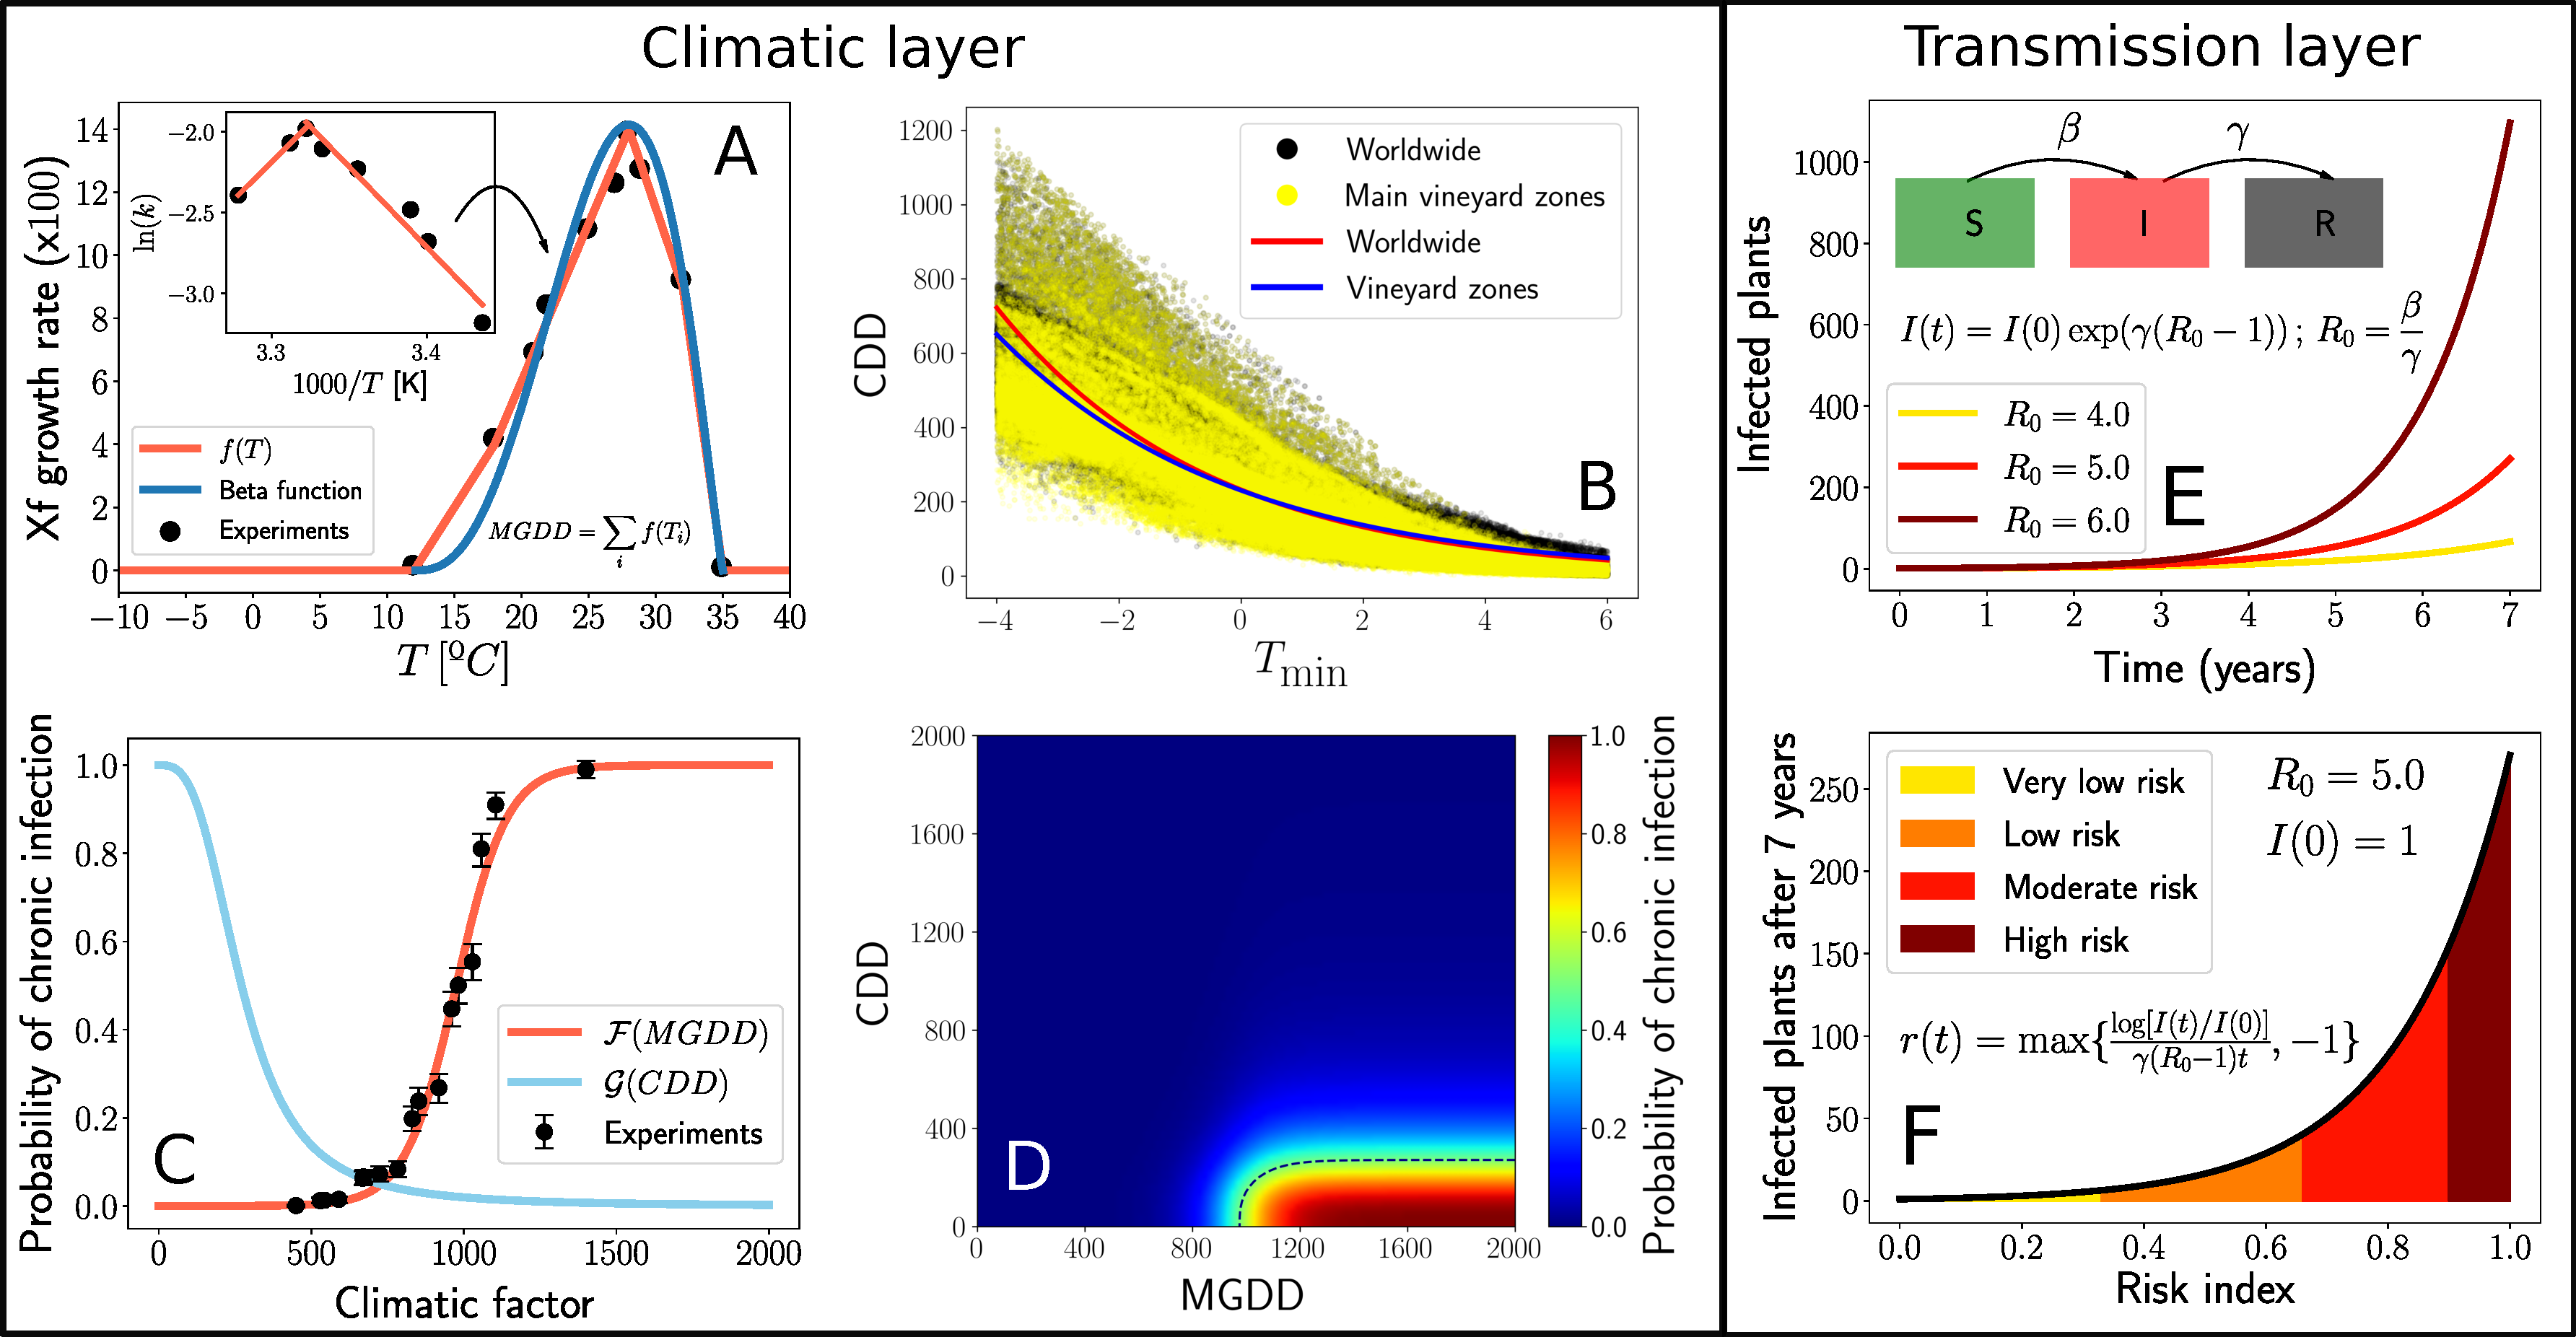
\includegraphics[width=\textwidth]{Figures/Model_h.pdf}
    \caption{\textbf{Climatic and transmission layers composing the
            epidemiological model}. (\textbf{A}) $MGDD$ profile fitted to the
        \textit{in
            vitro } data of Xf growth rate in Feil \& Purcell 2001
        \cite{Feil2001}. The
        original Arrhenius plot in Kelvin degrees (inset) was converted to
        Celsius, as
        explained in Online Supplementary Information, to obtain the main plot.
        (\textbf{B})
        Correlation between CDD and the average $T_{\textrm{min}}$ of the
        coldest month
        between 1981 and 2019. Plotted black dots (worldwide) and yellow dots
        (main
        wine-producing zones) depict climatic data from 6,487,200 cells at
        $\SI{0.1}{\degree} \cross \SI{0.1}{\degree}$ resolution, spread
        globally and
        retrieved from ERA5-Land dataset. The red solid line depicts the fitted
        exponential function for worldwide data and the blue solid line for
        main
        vineyard zones. (\textbf{C}) Nonlinear relationship between MGDD (red
        line) and
        CDD (blue line) and the likelihood of developing chronic infections.
        Black dots
        depict the cumulative proportion of grapevine plants in the population
        of $36$
        inoculated varieties showing five or more symptomatic leaves at each of
        the 15
        $MGDD$ levels (see Online Supplementary Information). Vertical bars are
        the
        95\% CI.
        (\textbf{D}) Combined ranges of $MGDD$ and $CDD$ on the likelihood of
        developing chronic infection. (\textbf{E}) Transmission layer in the
        dynamic
        equation (1) of the SIR compartmental model. (\textbf{F}) Relationship
        between
        the exponential growth of the number of infected plants with the risk
        index and
        their ranks.}
    \label{fig1}
\end{figure*}

\subsection{Thermal requirements to develop PD.}
We examined the response
of a wide spectrum of European grapevine varieties to Xf$_{\textrm{PD}}$
infection in three independent experiments conducted in 2018, 2019, and 2020.
Overall, 86.1\% ($n$ = 764) of 886 inoculated plants, comprising 36 varieties
and 57 unique scion/rootstock combinations, developed PD symptoms 16 weeks
after inoculation. European \textit{V. vinifera} varieties exhibited
significant differences in their susceptibility to Xf$_{\textrm{PD}}$
(Online Supplementary Information). All varieties, however, showed PD symptoms
to some
extent,
confirming previous field observations of general susceptibility to
Xf$_{\textrm{PD}}$ \cite{Hopkins2002, Moralejo2019, Purcell2013}.  We also
found significant differences in virulence ($\chi^2=68.73$, $\textrm{df}=1$,
$P=2.2 \cross 10^{-16}$) between two Xf$_{\textrm{PD}}$ strains isolated from
grapevines in Majorca across grapevine varieties (\cref{figS1}). Full details
on the results of the inoculation tests are available in Methods and
Supplementary
Information.

Growing degree days (GDD) have traditionally been used to describe and predict
phenological events of plants and insect pests, but rarely in plant diseases
\cite{McMaster1997}. We took advantage of data collated in the inoculation
trials together with temperature to relate symptom development to the
accumulated heat units at weeks eight, 10, 12, 14 and 16 after inoculation
(Supplementary Data 1).  Rather than counting GDDs linearly above a threshold
temperature, we consider Xf's specific growth rate \textit{in vitro} within its
cardinal temperatures. The empirical growth rates come from the seminal work by
Feil \& Purcell \cite{Feil2001} shown in the inset of \cref{fig1}A. This
Arrhenius plot is transformed, as explained in Online Supplementary
Information, to obtain a
linear approximation in a limited range of temperatures as shown in the main
plot of \cref{fig1}A. Inspired by the fit in Fig. 3 of \cite{Feil2001}, we
approximate the growth rates by a piece-wise function $f(T )$ (see Methods
below) formed by four segments. This Modified Growing Degree Day (MGDD) profile
\label{eq:MGDD_def} enables to measure the thermal integral from hourly average
temperatures, improving the prediction scale of the biological process
\cite{butikofer2020problem}. MGDD also provides an excellent metric to link
Xf$_{\textrm{PD}}$ growth in culture with PD development as, once the pathogen
is injected into the healthy vine, symptoms progression mainly depends upon the
bacterial load (i.e., multiplication) and the movement through the xylem vessel
network, which are fundamentally temperature-dependent processes
\cite{fry1990multiplication,Feil2001}. Moreover, MGDD can be mathematically
related to the exponential or logistic growth of the pathogen within the plant
(Online Supplementary Information).

Interannual infection survival in grapevines plays a relevant role when
modelling PD epidemiology. In our model, we assumed a threshold of five or more
symptomatic leaves for these chronic infections based on the relationship
between the timing and severity of the infection during the growing season and
the likelihood of winter recovery  \cite{Feil2001, Feil2003, Lieth2011}. This
five-leaf cut-off was grounded on: (i) the bimodal distribution in the
frequency of the number of symptomatic leaves among the population of
inoculated grapevines (\cref{figS1}), whereby vines that generally show less
than five symptomatic leaves at 12 weeks after inoculation remain so in the
following weeks, while those that pass that threshold continue to produce
symptomatic leaves, and (ii) the observed correlation between the acropetal and
basipetal movement of Xf along the cane (\cref{figS1}). The likelihood of
developing chronic infections as a function of accumulated MGDD among the
population of grapevine varieties was modelled using survival analysis with
data fitted to a logistic distribution $\mathcal{F}(MGDD)$. A minimum window of
$MGDD=528$ was needed to develop chronic infections (var. Tempranillo), about
975 for a median estimate, while a cumulative $MGDD>1159$ indicate over 90\%
probability within a growing season (red curve in \cref{fig1}C and Methods).

Next, we intended to model the probability of disease recovery by exposure to
cold temperatures. Previous works had specifically modelled cold curing on
Pinot Noir and Cabernet Sauvignon varieties in California as the effect of
temperature and duration \cite{Lieth2011} by assuming a progressive elimination
of the bacterial load with cold temperatures \cite{Feil2003}. In the absence of
appropriate empirical data to formulate a general average pattern of winter
curing among grapevine varieties, we combined the approach of Lieth et al.
\cite{Lieth2011} and the empirical observations of Purcell on the distribution
of PD in the US related to the average minimum temperature of the coldest
month, $T_{min}$, isolines \cite{Anas2008}. To consider
the accumulation of cold units in an analogy of the MGDD, we searched for a
general correlation between $T_{min}$ and the cold degree days (CDDs) with base
temperature = $6$ \textdegree C (see Methods). We found an exponential
relation, $CDD \sim 230\exp(-0.26\cdot T_{\textrm{min}})$, where specifically,
$CDD\gtrsim306$ correspond to $T_{\textrm{min}}<\SI{-1.1}{\degree C}$
\cref{fig1}B. To transform this exponential relationship to a probabilistic
function analogous to $\mathcal{F}(MGDD)$, hereafter denoted
$\mathcal{G}(CDD)$, ranging between 0 and 1, we considered the sigmoidal family
of functions $\displaystyle f(x)=\frac{A}{B+x^C}$ with $A=9\cdot 10^6$, $B=A$
and $C=3$ (\cref{fig1}C), fulfilling the limit $\mathcal{G}(CDD=0)=1$, i.e. no
winter curing when no cold accumulated, and a conservative 75\% of the infected
plants recovered at $T_{\textrm{min}}=\SI{-1.1}{\degree C}$ instead of 100\% to
reflect uncertainties on the effect of winter curing.

\subsection{MGDD/CDD distribution maps.}
MGDD were used to compute annual
risk maps of developing PD during summer for the period 1981-2019 (see
Methods). The resulting averaged map identifies all known areas with a
recent
history of severe PD in the US corresponding to $\mathcal{F}(MGDD) > 90\%$
(i.e., high-risk), such as the Gulf Coast states (Texas, Alabama,
Mississippi,
Louisiana, Florida), Georgia and Southern California sites (e.g., Temecula
Valley) (\cref{fig2}\textit{A}), while captures areas with a steep
gradation of
disease endemicity in the north coast of California ($\mathcal{F}(MGDD >
    50\%$). Overall, more than $95\%$ of confirmed PD sites ($n = 155$) in
    the
    US (Supplementary Data 2) fall in grid cells with $\mathcal{F}(MGDD) >
50 \%$.

    The average MGDD-projected map for Europe during 1981-2019 spots a high
    risk
    for the coast, islands and major river valleys of the Mediterranean Basin,
    southern Spain, the Atlantic coast from Gibraltar to Oporto, and
    continental
    areas of central and southeast Europe (\cref{fig2}B). Of these, however,
    only
    some Mediterranean islands, such as Cyprus and Crete, show
$\mathcal{F}(MGDD) >
99\%$ comparable to areas with high disease incidence in the Gulf Coast states
    of the US and California. Almost all the Atlantic coast from Oporto
    (Portugal)
    to Denmark are below suitable $MGDD$, with an important exception in the
    Garonne river basin in France (Bordeaux Area) with low to moderate $MGDD$
    (\cref{fig2}B).

    \cref{fig2}A shows how the area with high-risk MGDD values extends further
    north of the current known PD distribution in the southeastern US,
    suggesting
    that winter temperatures limit the expansion of PD northwards
    \cite{Hopkins2002}. A comparison between MGDD and CDD maps (\cref{fig2}A
    vs.
    \cref{fig2}C, \cref{fig2}E) further supports the idea that winter curing is
    restricting PD northward migration from the southeastern US. However,
    consistent with growing concern among Midwest states winegrowers on PD
    northward migration led by climate change \cite{Galvez2010}, we found a
    mean
    increase of $0.12 \%$ y$^{-1}$ in the areal extent with $CDD < 306$ ($\sim
T_{\textrm{min}} < -1.1$ \textdegree C) since 1981, comprising land areas
    between $103^o$W and $70^o$W of the US (\cref{fig:sup_CDD_evol}). Such an
    upward trend corresponds to $\SI{5090}{km^2}$ y$^{-1}$ in the potential
    northward expansion of PD due to climate change and an accumulation of
$\sim\SI{193420}{km^2}$ of new areas at risk since 1981.

    High-CDD values would also be expected to restrict the potential PD
    colonisation in continental Europe (\cref{fig2}D). Unlike North America,
    the
    East-West distribution of major European mountain ranges together with the
    warming effect of the Gulf Stream decreases the likelihood of cold winter
    spells reaching the western Mediterranean coast. $\mathcal{G}(CDD)$ between
    100\% and 95\% (i.e., recovery probability $<5\%$ -- low winter curing) are
    mostly prevalent below $40^o$N latitude in the southwest Iberian Peninsula
    and
    Mediterranean islands and coastlands ($<\SI{50}{km}$ away). Above $40^o$N
    latitudes, $CDD < 100$ are encountered mainly in the Atlantic coast and
    Mediterranean coast and islands (\cref{fig2}D). In contrast, central and
    southeast Europe show high CDD values likely preventing Xf$_{\textrm{PD}}$
    winter survival on infected grapevines.

    In \cref{fig2}E-F, we show the average climatic suitability for PD
    establishment only from the mechanistic relation between Xf$_{\textrm{PD}}$
    and
    temperature. Although all areas with current Xf$_{\textrm{PD}}$-related
    outbreaks are identified, risk predictions based only on the combination of
    MGDD and CDD could lead to overestimations, as this approach overlooks
    disease
    transmission dynamics and climate interannual variability.

    \begin{figure}[H]
        \centering
        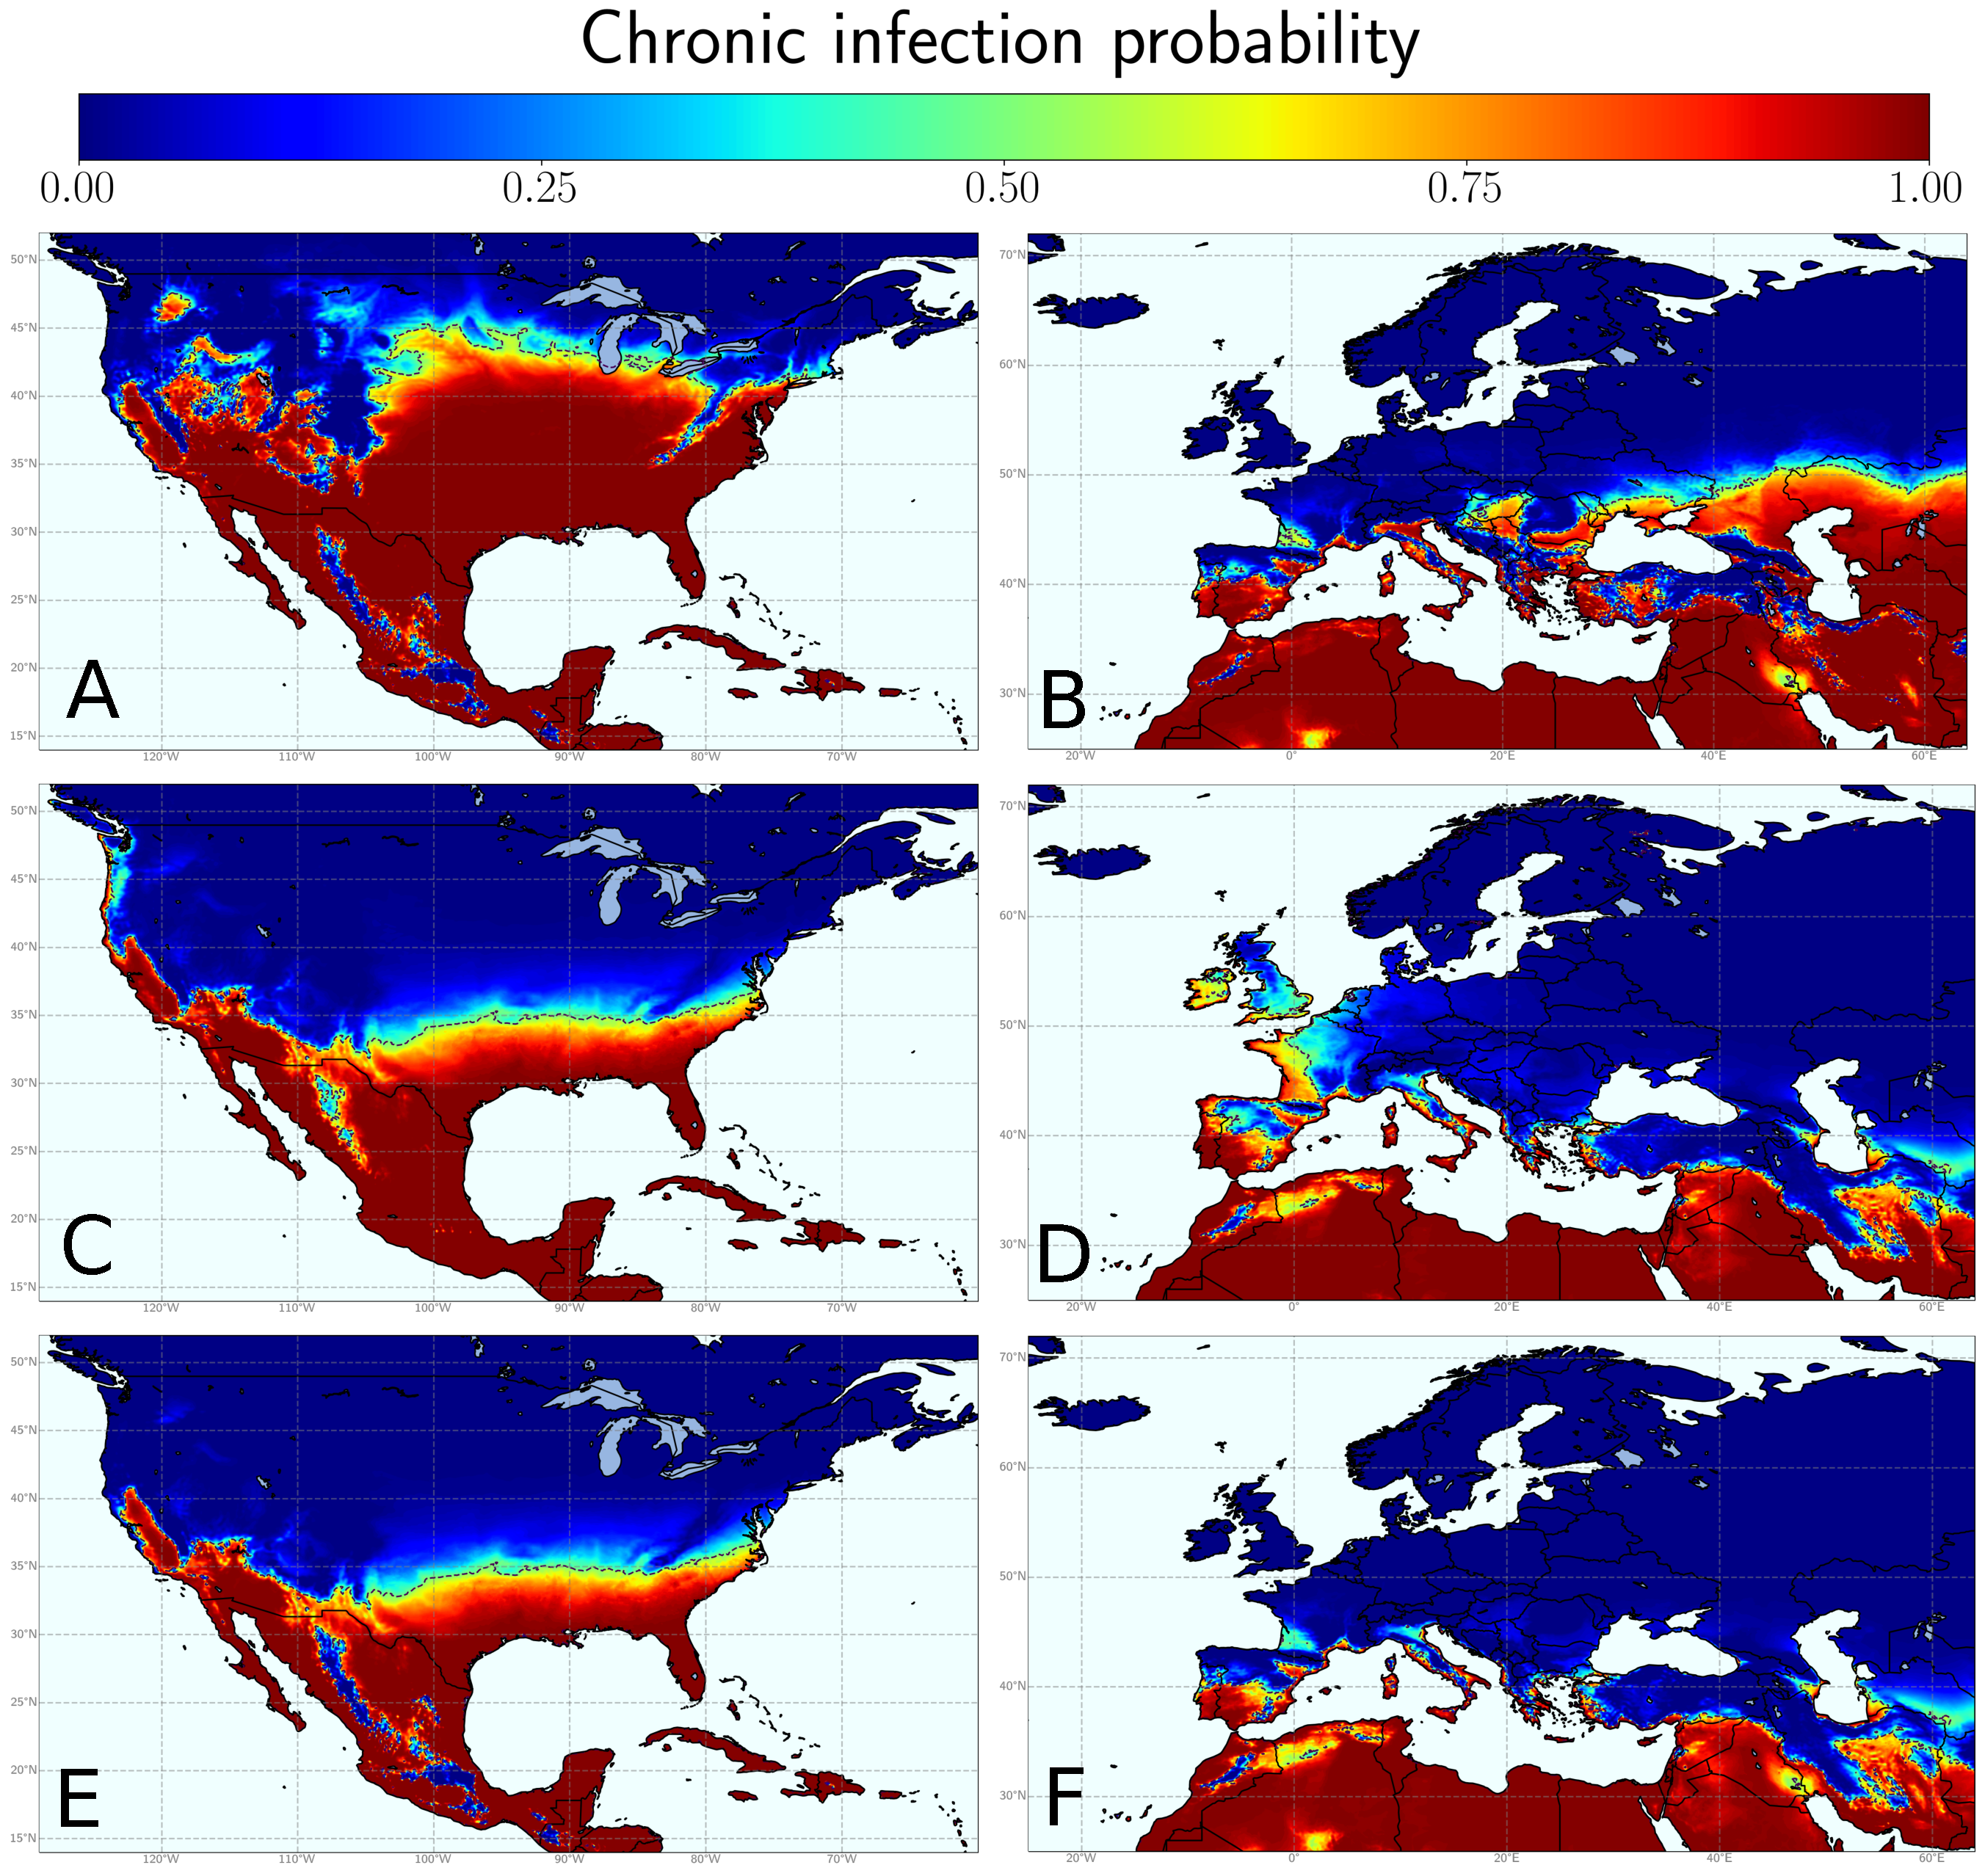
\includegraphics[width=0.85\textwidth]{Figures/Fig1_new.pdf}
        \caption{\textbf{Average thermal-dependent maps for Pierce's disease
                (PD)
                development and recovery in North America and Europe.} PD
            development during
            the growing season based on average $\mathcal{F}(MGDD)$ estimations
            between
            1981 and 2019 in North America (\textbf{A}) and Europe (\textbf{B})
            derived
            from the results of the inoculation experiments on 36 grapevine
            varieties.
            Large differences in the areal extension with favourable MGDDs can
            be observed
            between the US and Europe. The winter curing effect is reflected in
            the
            distribution of the average $\mathcal{G}(CDD)$ for the 1981-2019
            period in the
            United States (\textbf{C}) and Europe (\textbf{D}). A snapshot of
            the
            temperature-driven probability of chronic infection averaged for
            the 1981-2019
            period is obtained from the joint effect of MGDD and CDD in North
            America
            (\textbf{E}) and Europe (\textbf{F}). Warmer colours indicate more
            favourable
            conditions for chronic PD and the dashed line highlights the
            threshold of
            chronic infection probability being $0.5$.}
        \label{fig2}
    \end{figure}

    \begin{figure*}[t!]
        \centering
        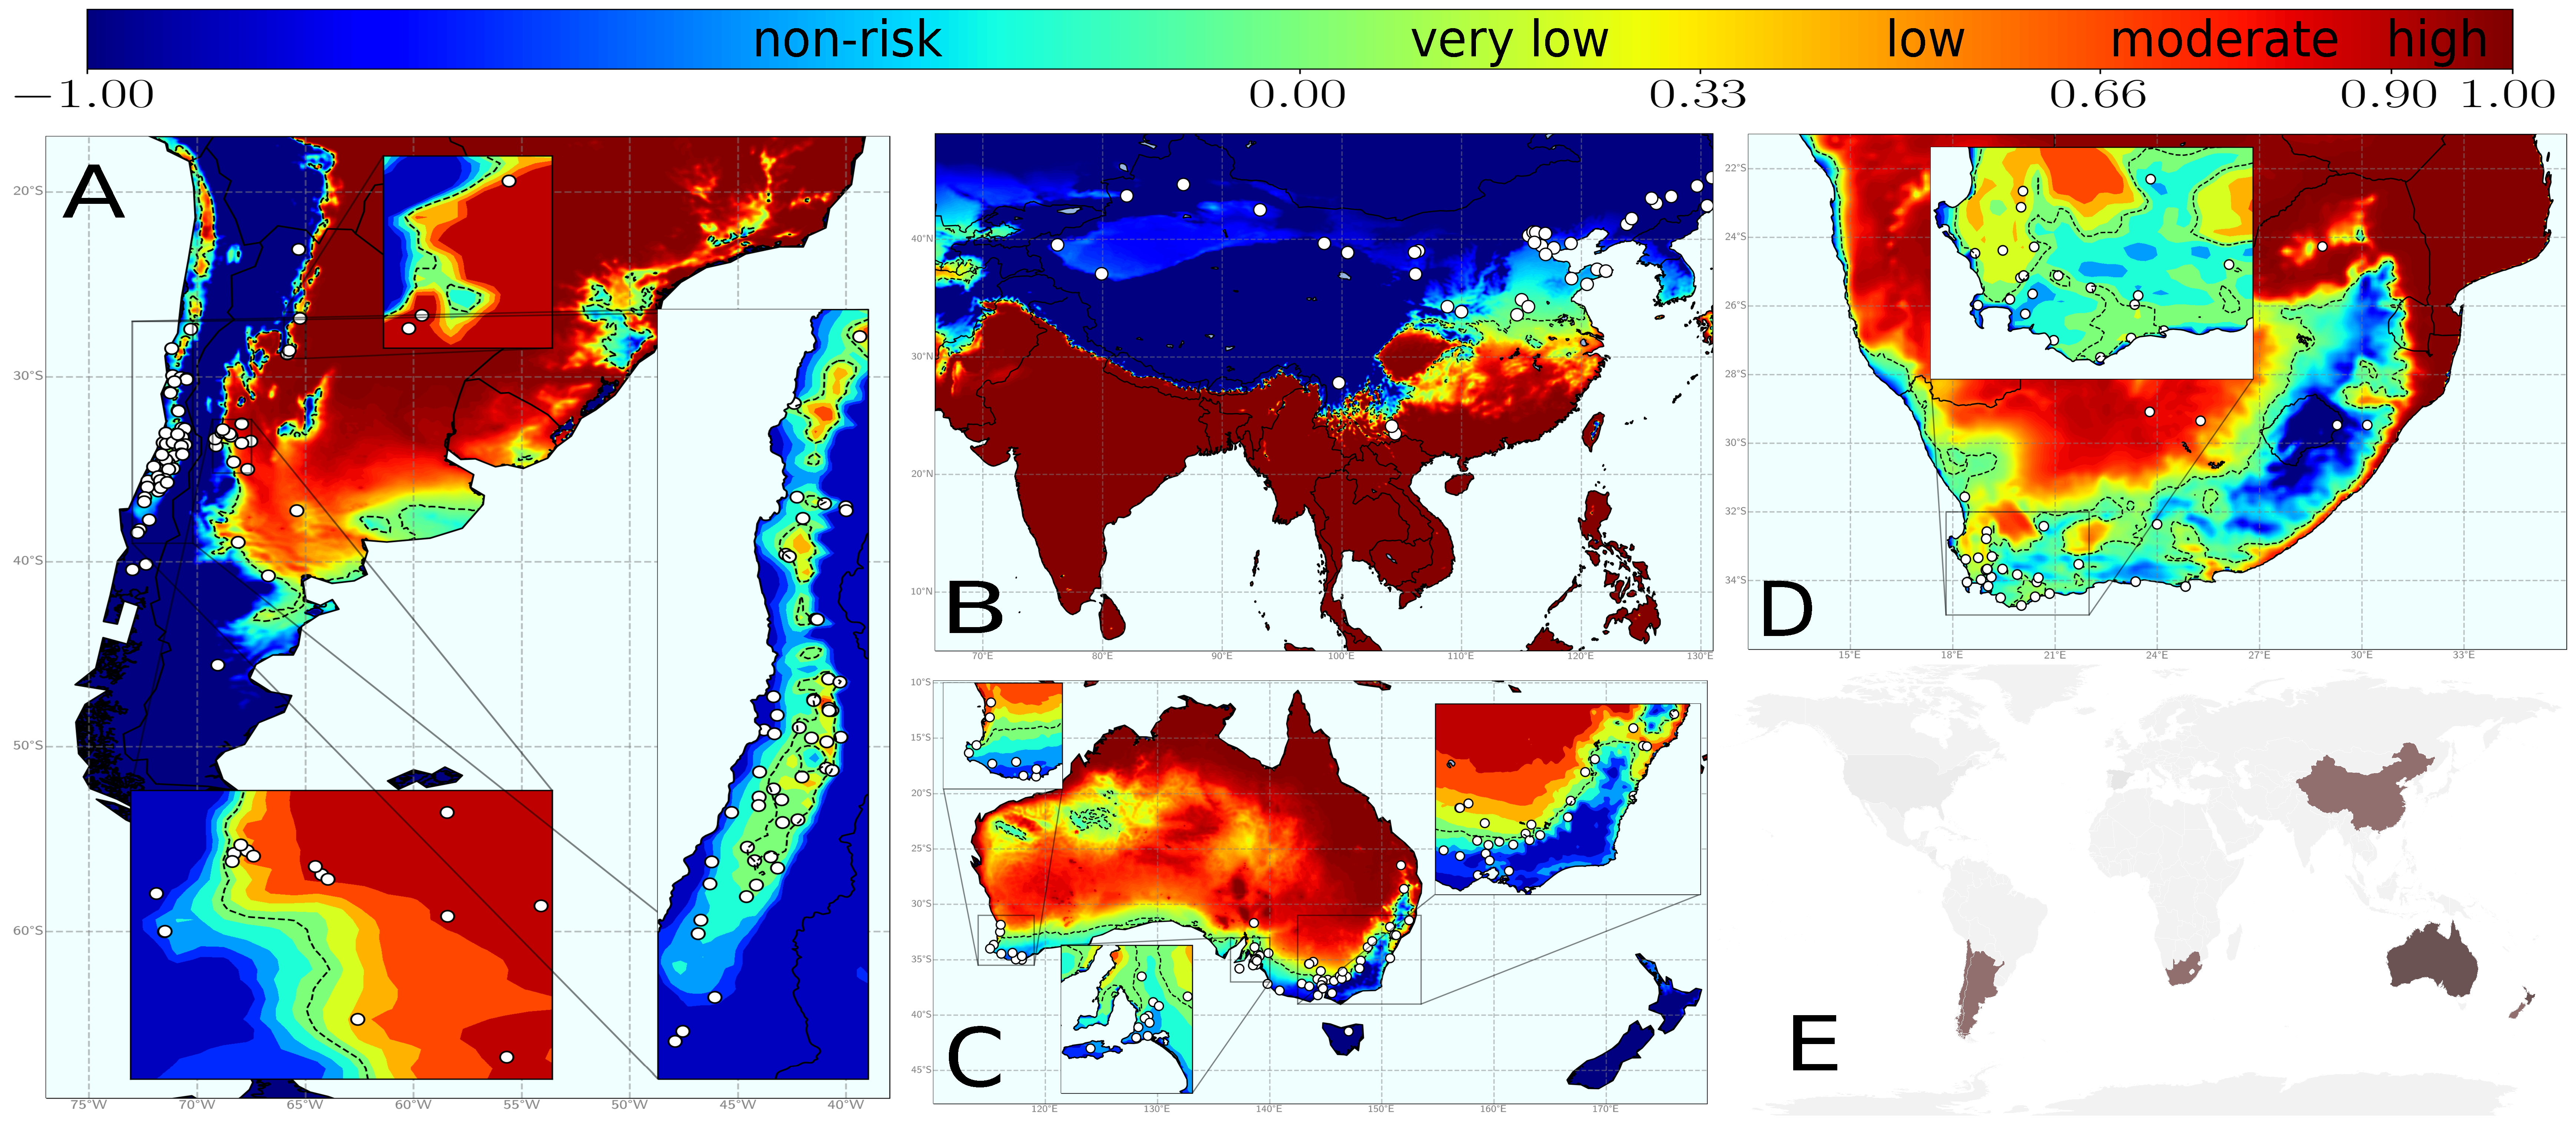
\includegraphics[width=1\textwidth]{Figures/Fig_global_risk_R0_5.pdf}
        \caption{\textbf{Climate-driven risk maps for PD establishment in main
                viticulture regions worldwide under a baseline $R_0 = 5$
                scenario.} White dots
            indicate the main vineyard areas in the wine-growing regions of
            China and the
            Southern Hemisphere. (\textbf{A}) Chile and Argentina; (\textbf{B})
            Asia with
            special attention to China; (\textbf{C}) Australia and New Zealand
            (wine areas
            are not marked as the whole country is without risk); and
            (\textbf{D}) South
            Africa. (\textbf{E}) Global distribution of main wine-producing
            areas analysed.
            The risk index $r_j(t)$, express the relative exponential growth
            rate of the
            disease incidence, and was scaled from 0.1 to 1 and ranked as very
            low
            (0.10-0.33), low (0.33-0.66), moderate (0.66-0.90) and high ($>
                0.90$).}
        \label{fig3}
    \end{figure*}

    \subsection{PD global risk.}
    We ran several simulations of the model \cref{eq:evolution_eq} with $R_0$
    values between 1 and 14 to validate PD spatiotemporal distribution in the
    US.
    We found $R_0=8$ as the optimal parameter for maximising the area under a
    ROC
    curve (\cref{fig:sup_ROC}), returning an accuracy of more than $80 \%$,
    except
    for 2006, due to data obtained from an area at the transient-risk zone
    (\cref{fig:sup_validation} and \cref{tab:validation}). For Europe and the
    rest
    of the world, we derived a $R_0=5$, as a maximal baseline estimate for
    modelling PD transmission (see Methods and Online Supplementary
    Information). These
$R_0$
    values should be taken as operating estimates for the model.  From the
    model
    simulations \cref{eq:evolution_eq}, we obtained a risk index $r$ that
    measures
    the relative exponential growth rate in the population of infected plants
    at
    the epidemic onset with respect to the maximum growth, $r=1$. This index
    served
    to rank the epidemic-risk zones in high ($> 0.9$), moderate ($0.66-0.9$),
    low
    ($0.33-0.66$) and very low ($\sim 0.075-0.33$) risks (see \cref{fig1}F,
    Methods, and Online Supplementary Information).

    \begin{table}[H]
        \begin{center}
            \caption{\textbf{Validation of model predictions.} The items are
                locations
                where PD was present or absent. TP corresponds to true
                positives and TN to true
                negatives according to our model with $R_0=8$. }
            \label{tab:validation}
            \resizebox{0.8\textwidth}{!}{%
                \begin{tabular}{llllll}
                    \hline
                    Year  & Presence & Absence & TP & TN & Accuracy \\
                    \hline
                    2001  & 16       & 5       & 15 & 3  & 86\%     \\
                    2002  & 12       & 2       & 11 & 1  & 86\%     \\
                    2005  & 4        & 2       & 4  & 1  & 83\%     \\
                    2006  & 8        & 0       & 4  & 0  & 50\%     \\
                    2015  & 53       & 0       & 51 & 0  & 96\%     \\
                    \hdashline
                    TOTAL & 93       & 9       & 85 & 5  & 88\%     \\
                    \hline
                \end{tabular}
            }
        \end{center}
    \end{table}

    To date, PD is mainly restricted to the American continent with some
    unrelated
    introductions of Xf$_{\textrm{PD}}$ to Taiwan and Majorca (Spain) from the
    United States \cite{Moralejo2019,Su2013}. To assess the risk of PD
    establishment elsewhere, we projected our epidemiological model into the
    main
    winegrowing regions of the Northern Hemisphere (US, Europe and China) and
    Southern Hemisphere (Chile, Argentina, South Africa, Australia and New
    Zealand)(\cref{fig3}A-E). We found that emerging wine-producing areas in
    China
    are predominantly located in non-risk zones, whereas only some vineyards in
    the
    Henan and Yunnan provinces fall in transition and moderate-high risk zones
    (\cref{fig3}B and Supplementary Data 3). In Europe, 92.1\% of the territory
    is
    in non-risk zones and 6.1\% is included in the epidemic-risk zone, with
    only
    1.9\% showing a high-risk index and 1.5\% a moderate risk
    (Online Supplementary Information).
    The model also reveals a progressive transition from areas without risk
    ($r(t)
< 0$) before 1990 to epidemic-risk zones with low-risk indexes by 2019
    (\cite{Webpage}, see Movies), mainly affecting the basins of the rivers Po
    in
    Italy, Garonne and Rhone in France and Douro/Duero in Portugal and Spain.
    This
    represents a mean increase of $0.21\%$ y$^{-1}$ in the epidemic-risk zone,
    a
    rate $3.5$-times greater than that of the eastern US, which could increase
    the
    likelihood of PD establishment in Europe in the coming decades. In the US,
    most
    states around the Gulf Coast show high-risk indexes, whereas, around 37.5\%
    of
    California's surface is suitable for epidemics with high growth rate
    incidence
    (Online Supplementary Information).

    In the Southern Hemisphere, vineyards at non-risk or transient
    epidemic-risk
    zones predominate -- e.g., non-risk in New Zealand and Tasmania
    (\cref{fig3}C).
    Risk indexes in areas where PD can become established ($r(t) > 0$) range
    from
    very low to low for most coastal vineyards in Australia (west, south and
    east)
    with somehow more suitable conditions in the interior of New South Wales,
    Greater Perth and Queensland (\cref{fig3}C); a general very-low or low-risk
    indexes are predicted in the Western Cape in South Africa (\cref{fig3}D);
    overall very-low but localised low to moderate risk indexes in some areas
    in
    Chile; and low to moderate growth of the number of infected vines in most
    of
    Argentina, being this the wine-growing country with the highest risk
    (\cref{fig3}A). Detailed information on areas with non-risk, transient risk
    and
    risk indexes (i.e., disease-incidence growth rates) in areas with the
    potential
    risk of establishment by country and regions is provided in Supplementary
    Information.

    \begin{figure}[H]
        \centering
        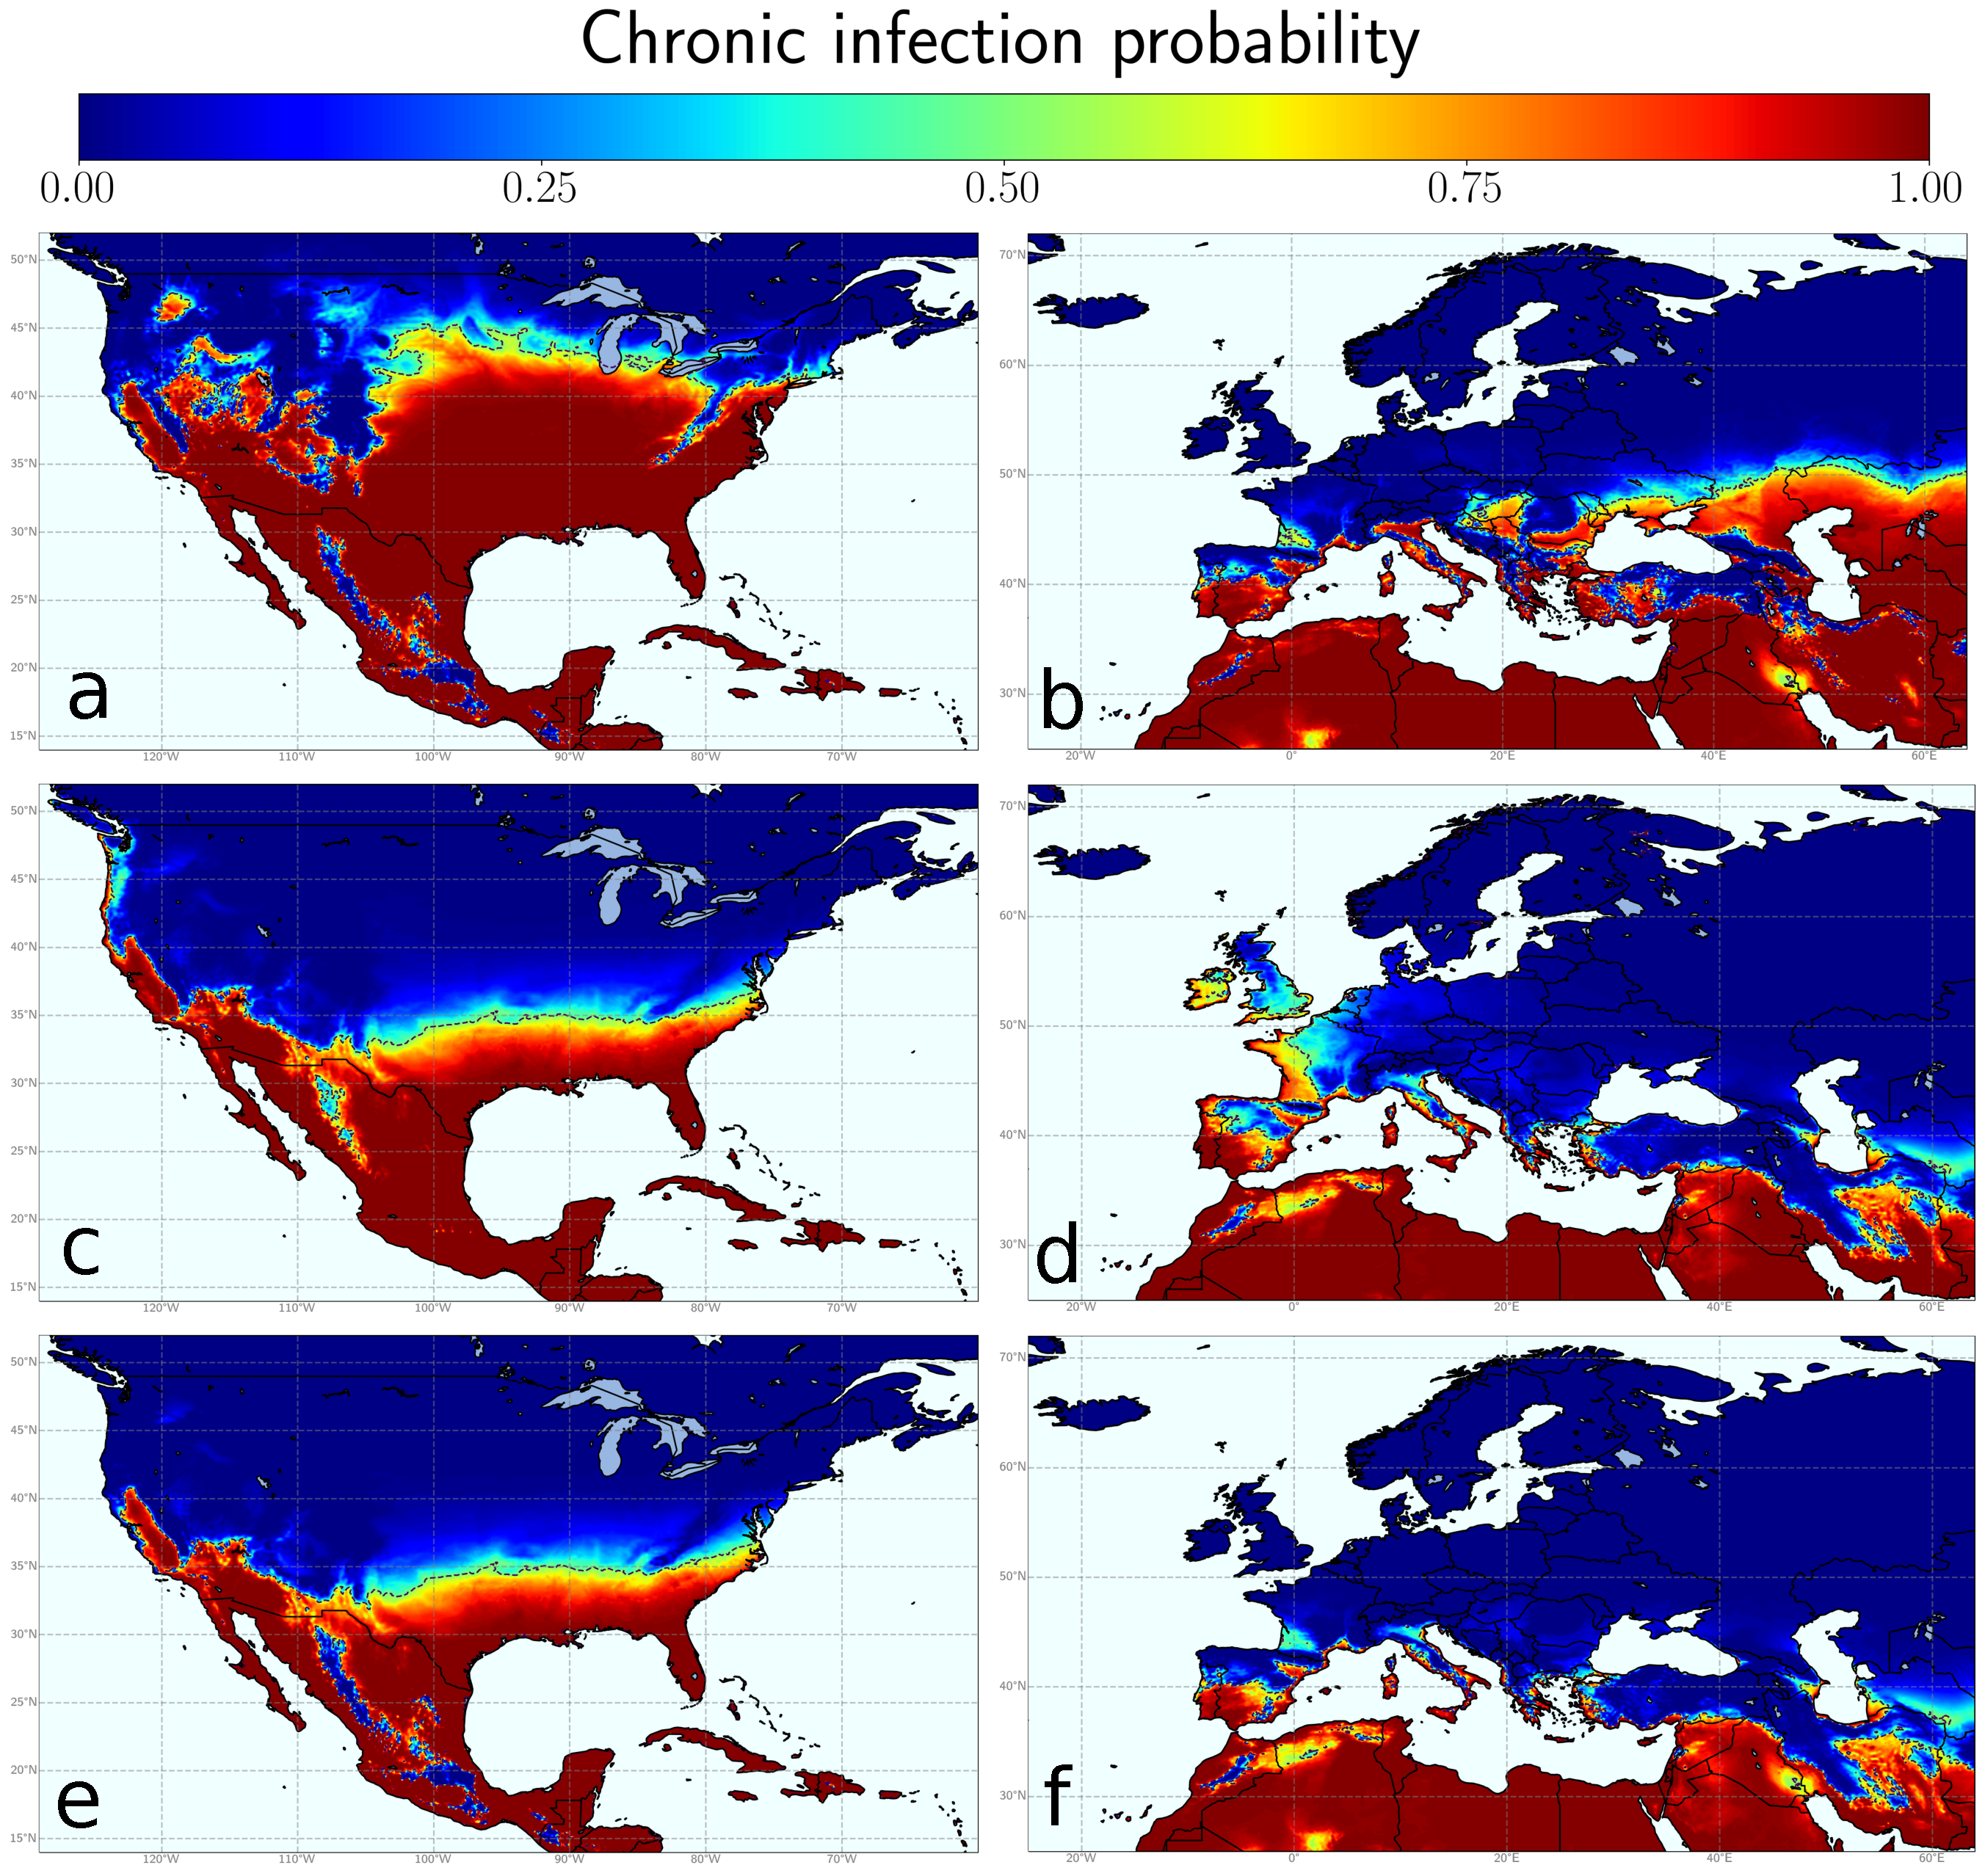
\includegraphics[width=0.9\textwidth]{Figures/Fig2.pdf}
        \caption{\textbf{Temperature-driven dynamic-model simulations  for PD
                establishment from 1981 to 2019 under different $R_0$ scenarios
                with a
                spatially homogeneous vector distribution.} For comparison, the
            baseline
            scenario with a $R_0=5$ for Europe is projected to North America
            (\textbf{A})
            capturing to some extent the distribution and severity of PD in
            that continent.
            In Europe (\textbf{B}) high-risk areas (i.e., $r_j(t) > 0.90$) are
            restricted
            to coastal Mediterranean and the south of the Iberian Peninsula;
            black dash
            line separate areas with $r(t)>0$ where theoretically PD can
            thrive. Under
            higher $R_0$ scenarios, $R_0=8$ for North America (\textbf{C}) and
            Europe
            (\textbf{D}), the dash lines tend to separate from isoline
            $T_{\textrm{min}} =
                -1.1$\textdegree C (white line); and even more in extreme
            transmission pressure
            $R_0=16$ for North America (\textbf{E}) and Europe (\textbf{F}). }
        \label{fig4}
    \end{figure}

    Risk indexes may vary within epidemic-risk zones if any of the
    epidemiological
    parameters governing transmission change. As expected, $I(t) < I(0)$
    boundaries
    increasingly displace to northern latitudes in the US and Europe under
    higher
    transmission scenarios, increasing the risk-epidemic zones significantly
    (\cref{fig4}A-F). The line representing the outbreak extinction i.e., the
    non-risk zone $r(t)<-0.09$, in the validated $R_0=8$ scenario for the US,
    falls
    at some distance above the isoline $T_{\textrm{min}} = -1.1^o$C in
    comparison
    to the $R_0=5$ scenario (\cref{fig4}, \cite{Webpage}). This distribution
    pattern holds and moves slightly northward over
    time
    in parallel to global warming, although the trend of PD latitudinal change
    is
    moderated by high-CDD values (i.e. cold accumulation). In addition, the
    disease
    extension also declines due to CDD interannual fluctuations in the
    simulations.
    Cold waves periodically occur that reach latitudes close to the Gulf, such
    as
    those that occurred in 1983, 1993, 1995, 2000, 2009 and 2013 (Movies at
    \cite{Webpage}), thus preventing PD expansion northward. The magnitude of
    this
    decrease is revealed after comparing the average annual increase of the
    areas
    between $r(t) > 0$ and $CDD < 306$ lines. From 1981 to 2019, the area with
    risk
$r(t) > 0$ increased at a rate of $0.05\%$ y$^{-1}$, while that of $CDD < 306$
    by $0.12\%$ y$^{-1}$, an important difference not explained alone by CDDs
    without considering climate fluctuations (\cref{fig:sup_CDD_evol}).

    \subsection{PD risk projections for 2050}. Global shifts in the risk
    index
$r_j(t)$ between 2019 and those projected for 2050 were calculated under the
    same baseline scenario (\cref{fig5}A-F, Methods). Our simulation shows a
    generalised increasing trend mainly due to shifts from transition zones to
    epidemic-risk zones with very low or low-risk indexes in the main
    wine-growing
    regions, except for the US. Here the epidemic-risk zone would increase by
$12.8\%$ with the greater increments in the high-risk index category ($22.7\%$)
    and a decrease in the transition zones (Online Supplementary Information).
    Much
    less surface
    would be included in the epidemic-risk zone in Europe ($8.6\%$) compared to
    the
    US ($36.5\%$). However, the epidemic-risk zone would expand by $40.0\%$
    with
    respect to 2020, a rate more than three times higher than that of the US
    (Online Supplementary Information). Such increases are due to the emergence
    of
    previously
    unaffected areas in 2020 evolving into epidemic-risk zones by 2050, and
    epidemic growth-rate increases in already epidemic-risk zones in 12 of 42
    countries (Online Supplementary Information). Among these 12 countries,
    however,
    there is
    substantial variation in the risk index increments within epidemic-risk
    zones
    with respect to 2019 (Online Supplementary Information). While non-risk
    zones
    still cover
$87.6\%$ of Europe's land area, epidemic-risk zones with high-risk indexes are
    expected to be almost two-fold higher than that of 2019, comprising $3.2\%$
    of
    Europe (\cref{table2}). \\

    \begin{figure*}[b!]
        \centering

        \includegraphics[width=\textwidth]{Figures/Fig_global_risk_change_R0_5.pdf}
        \caption{\textbf{Global shifts in PD risk index ($r_j(t)$) from 2020 to
                2050.} To build the maps, we have assumed a spatial homogeneous
            vector
            distribution and a $R_0=5$ scenario, except for the US where a
            $R_0=8$ has been
            used in the model simulations.\textbf{(A)} North
            America;\textbf{(B)}
            Europe;\textbf{(C)} Asia; \textbf{(D)} South America; \textbf{(E)}
            Australia
            and New Zealand; and \textbf{(F)} South Africa. Risk-index
            increases are in red
            and decreases in blue. The dashed line represents the spatial
            threshold where
            $r_j(t)$ difference changes from negative to positive.}
        \label{fig5}
    \end{figure*}

    \begin{table*}[t!]
        \centering
        \caption{\textbf{Shifts in risk areas for Pierce's disease in Europe
                projected
                for 2050 under a $R_0$ = 5 scenario.} The model was run
            assuming the same
            homogeneous spatial distribution of the vector for the whole
            period.}
        \begin{tabular*}{\hsize}{@{\extracolsep{\fill}}lllllll}
            \hline
            Risk & 2050 & 2020 & Difference & Difference & 2050 & 2020 \\
            & km$^2$ & km$^2$ & km$^2$ & (\%) & (\%) area & (\%) area \\
            \hline
            No risk & $8885300.5$ & $9334178.7
            $ & $-448878.2
            $ & $-4.8
            $ & $87.6
            $ & $92.1
            $ \\
            Transition & $381081.3$
            & $182872.6$ & $198208.7$ & $108.3$ & $3.8$ & $1.8$ \\
            Very low & $189025.3$ & $179225.7
            $ & $9799.6$ & $5.5$ & $1.9$ & $1.8$ \\
            Low & $207599.4$ & $104143.1$ & $103456.3$ & $99.3$ & $2.1$ & $1.0$
            \\
            Moderate & $154780.5$ & $148621.4$ & $6159.0$ & $4.1$ & $1.5$ &
            $1.5$ \\
            High & $322225.9$ & $190971.4$ & $131254.5$ & $68.7$ & $3.2$ & $1.9
            $ \\
            \hline
        \end{tabular*}
        \label{table2}
    \end{table*}

    \subsection{Risk based on vector information}. So far, we have ignored
    the
    distribution of known and potential vector species due to their large
    number in
    the Americas and the limited quantitative information generally available.
    In
    the case of Europe, given \textit{P. spumarius} prevalence as a potential
    vector and its wide distribution, we added	a vector layer in a spatially
    dependent $R_0(j) = R_0^{\textrm{max}}\, v(j)$, where $v(j)$ is the
    climatic
    suitability for the vector (Methods), $v=1$ implies optimal climatic
    conditions
    with no constraints for the vector population size, while $v=0$ implies
    unsuitable climatic conditions and its absence (\cref{fig:sup_vector}).
    According to the model, no European zone shows a high-risk index and barely
$0.34\%$ of the territory falls in areas with potential moderate exponential
    growth rates in disease incidence (Online Supplementary Information).
    Irrespective
    of
    vineyard
    distribution, we estimated that PD could potentially become established
    (i.e.,
$r(t) > 0$) at a maximum of $3.1\%$ of the territory, while the area at
    moderate-risk index would be $5$-times lesser than the model without the
    vector's climate suitability layer, this latter more in consonance with
    other
    proposed risk maps \cite{Godefroid2019,Bragard2019}. Such differences in
    the
    projected risks are mainly concentrated in the warmest and driest
    Mediterranean
    regions and are due to uncertainties concerning temperature-humidity
    interactions in the ecology of the vector \cite{Godefroid2021}.

    \begin{figure*}[H]
        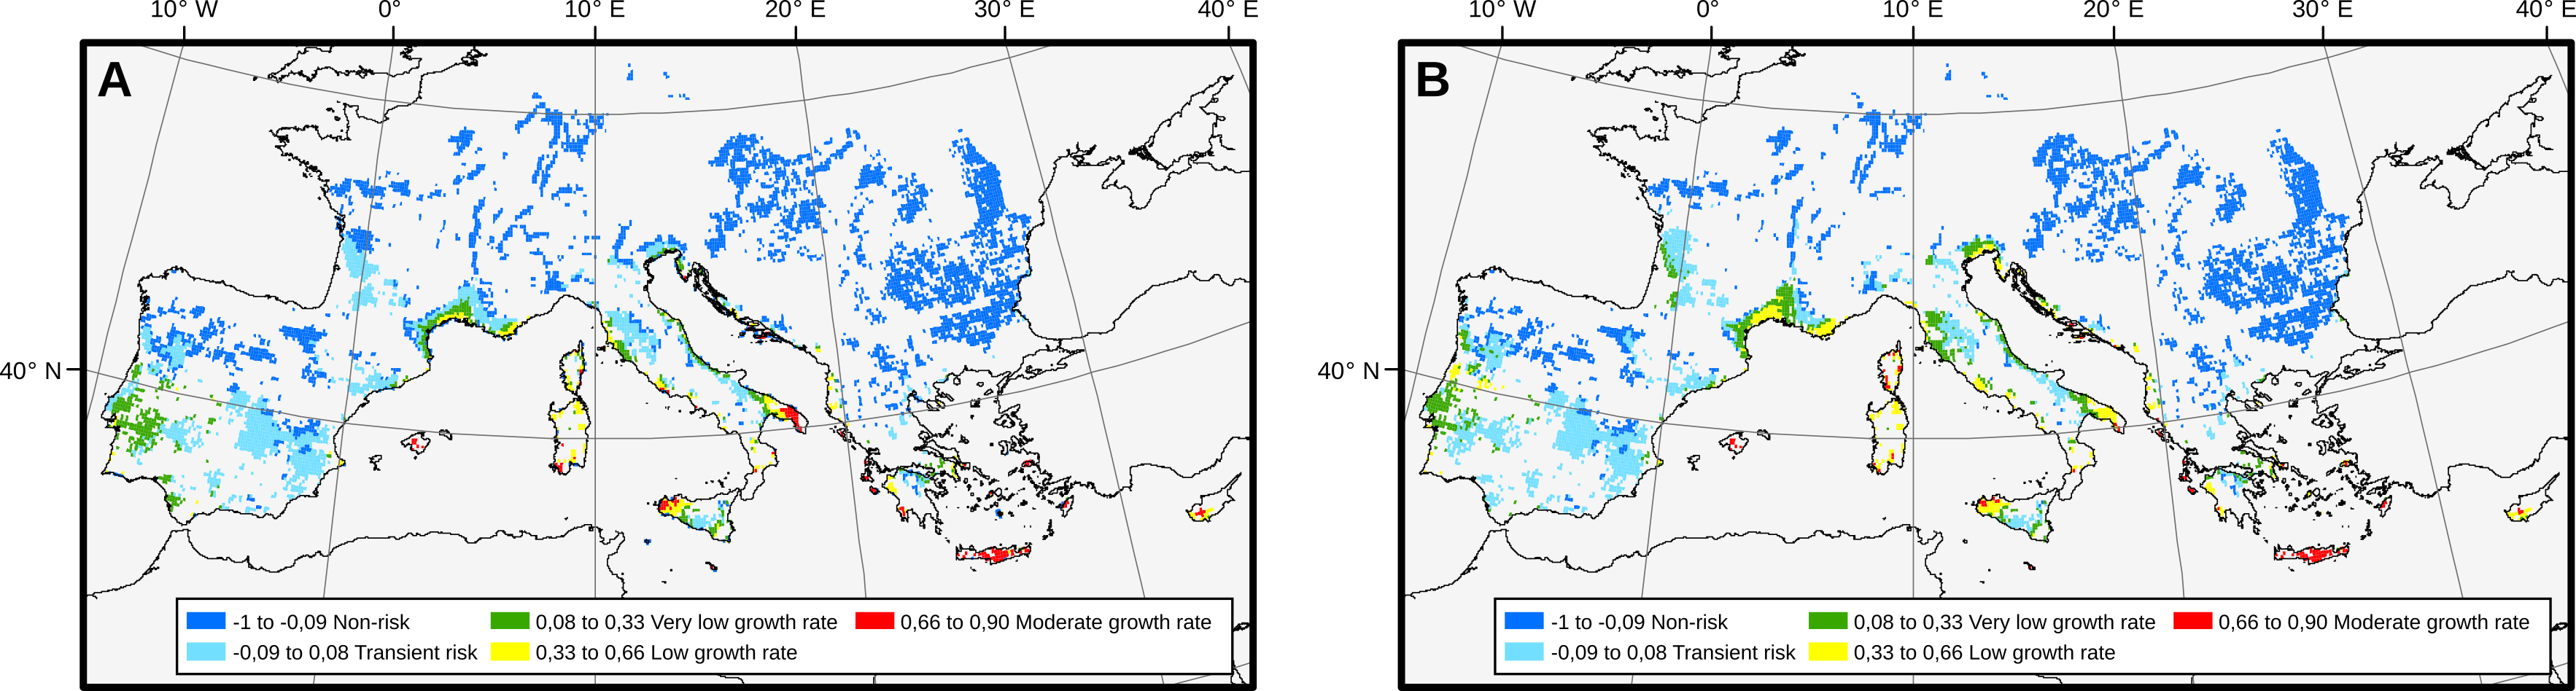
\includegraphics[width=1\textwidth]{Figures/vineyards.png}
        \caption{\textbf{Intersection between Corine-land-cover vineyard
                distribution map and PD-risk maps for 2020 and 2050.}  Data
            were obtained from
            Corine-land-cover (2018) and the layer of climatic suitability
            for\textit{P.
                spumarius} in Europe from \cite{Godefroid2021}. The surface of
            the vineyard
            contour has been enlarged to improve the visualisation of the risk
            zones and
            disease-incidence growth-rate ranks. \textbf{(A)} PD risk map for
            2019 and its
            projection for 2050 \textbf{(B)}. Blue colours represent non-risk
            zones and
            transient risk zones for chronic PD ($R_0 < 1$). The 2050 map shows
            some
            contraction of epidemic-risk zones with moderate risk indexes in
            Mediterranean
            islands and Apulia (Italy) as the climate becomes hotter and
            dryer.}
        \label{fig6}
    \end{figure*}

    \subsection{Combining vineyard land cover across Europe with the model
        output.}
    When we integrate into the model a layer of vineyard surface from
    Corine-Land-Cover, we find that PD could potentially become established
    (i.e.,
$r(t)>0.075$) in $22.3\%$ of the vineyards in Europe. However, no vineyard is
    in epidemic-risk zones with a high-risk index and only $2.9\%$ of the
    vineyard
    surface is at moderate risk (Online Supplementary Information). The areas
    with the
    highest
    risk
    index ($r(t)$ between $0.70$ and $0.88$) are mainly located in the
    Mediterranean islands of Crete, Cyprus and the Balearic Islands or at
    pronounced peninsulas like Apulia (Italy) and Peloponnese (Greece) in the
    continent (\cref{fig6}A and Online Supplementary Information).  Most
    vineyards are
    in
    non-risk
    zones ($42.1\%$), whereas $35.6\%$ are located in transition zones with
    presently non-risk but where Xf$_{\textrm{PD}}$ could become established in
    the
    next decades causing some sporadic outbreaks. In Online Supplementary
    Information,
    we provide full details of the total vineyard areas
    currently
    at risk for each country and region.

    Our model with climate and vector distribution projections for 2050
    indicates a
$ 55.8 \% $ increase in the epidemic-risk zone in Europe (\cref{fig6}B). This
    increment would be mainly due to the extension of epidemic-risk zones with
    very
    low and low-risk indexes. However, within the epidemic-risk zones, areas
    with
    moderate risk indexes would decrease from $\SI{114925}{ha}$ in 2020 to
$\SI{43114}{ha}$ in 2050, and no vineyards would be at high risk (\cref{fig6}B;
    see Online Supplementary Information). Counterintuitively, our
    model
    indicates a substantial increase in the area where PD could establish and
    become endemic for 2050, but a moderate decline in those areas where crop
    damage could be expected to be significant (e.g., Balearic Islands, Crete,
    Cyprus, Apulia).

    \section{Discussion}

    We introduce an epidemiological approach to assess the risk of PD
    establishment
    and epidemics in vineyards worldwide. The model includes the dynamics of
    the
    infected-host population, which enables estimating the initial exponential
    growth/decrease rate of the disease incidence. Unlike SDM correlative
    studies,
    Bayesian or, in general, machine learning black-box approaches, our model
    goes
    beyond by providing a mechanistic framework and thus explanatory power. In
    addition, it is flexible enough to simulate different climate and
    transmission
    scenarios, allowing, for instance, the incorporation of information on the
    spatial distribution of the vector. Comprehensive global PD risk maps
    result
    from the model simulations with historical climatic data. A web page is
    included, showing simulations with different parameters to estimate the
    risk of
    PD anywhere \cite{Webpage}.

    Temperature regulates key physiological processes of the ectothermic
    organisms
    involved in PD and thus limits the thermal range in which they can thrive
    \cite{Coakley1999}. Xf$_{\textrm{PD}}$ multiplication and survival within
    vine
    xylem vessels not only characterise PD, but also determine the bacterial
    population dynamics \cite{fry1990multiplication,Feil2001}. PD symptom
    development can be therefore characterised as a thermal-dependent
    continuous
    process within the range of  Xf$_{\textrm{PD}}$'s cardinal temperatures
    \cite{Scherm1994}. The combination of MGDD metrics with robust experimental
    data provides a reliable predictor of climatic suitability and the
    probability
    of developing PD during the summer, whereas CDD accounts for the effect of
    cold-temperature exposure on infected-plant recovery. This opposite
    contribution of MGDD and CDD in the demography of infected plants shapes
    the
    impact of climate variability on the epidemic dynamics in the early stages
    of
    the invasion (\cref{fig1}D). Given that the physiological basis of the
    plant-Xf
    interaction leading to symptoms development is poorly understood, we
    caution
    that other environmental factors, such as drought, nutrient status or crop
    management may modulate symptom expression and hence add an error in the
    MGDD
    parameter not measured in this work. Also, another limitation is that the
    relation between MGDD and Xf$_{\textrm{PD}}$ growth rates come from in
    vitro
    experiments and we assume that it is valid in planta as well. Nonetheless,
    we
    deem the error range would be smaller than the differences in the
    accumulated
$MGDD$s needed to reach the same disease level among varieties (i.e., regional
    differences) and smaller than the interannual $MGDD$ oscillations found in
    most
    locations.

    Knowledge of insect distribution is crucial for predicting epidemic
    outbreaks
    of endemic diseases, as well as the risk of invasion by emerging
    vector-borne
    pathogens (\cite {Caminade2017,Jeger2019}, (cf. \cite{Schneider2020})).
    Given
    the great diversity of known and potential vectors that can transmit PD
    \cite{Redak2004}, it has not been possible to include each region's
    particular
    vectors in the model. Therefore, when evaluating the risk of PD on a global
    scale, we have considered a homogeneous spatial distribution of the vector
    (fixed $ R_0 $), except in Europe where there is information on the main
    vector
    (\cref{fig:sup_vector}). As expected, the European case shows how models
    that
    assume a homogeneous spatial distribution of the vector generally produce
    epidemic risk zones with higher risk indexes than models that include a
    heterogeneous spatial distribution.
    This
    lack of information about vectors is one of the main reasons why the risk
    of
    vector-borne plant diseases is often overestimated.

    Risk overestimations may involuntarily stem from other additional sources
    too.
    Using mean data as inputs in epidemiological models can lead to biased
    results
    when response functions are nonlinear and climate variability is not
    accounted
    for \cite{Scherm1994}. This study presents experimental evidence of a
    non-linear relationship between MGDDs and PD chronic infections and
    indirect
    empirical evidence of a non-linear relationship between CDDs and PD
    recovery
    (\cref{fig:sup_climatic_oscilations}). Such a non-linear response
    consequently
    greatly impacts reducing the risk of PD establishment and steeping the
    spatial
    gradients in risk maps (\cref{fig4,fig6}). Moreover, MGDDs and CDDs might
    help
    to explain why disease pressure is much higher in the southeastern US than
    in
    California and Europe (\cref{fig2,fig4}) or, for example, earlier reports
    of PD
    outbreaks in Kosovo  \cite{Berisha1998}. Cooler summer nights in California
    and
    a shorter growing season compared to those found in the Gulf states in the
    southeastern US explain the difference in the accumulated $MGDD$ for both
    areas. In the case of Kosovo, $CDD$ values above certain thresholds could
    have
    led to the extinction of incipient outbreaks driven by several years with
$MGDD$ in the conducive range of PD (\cref{fig2}).

    Our PD risk map for Europe confirms previous predictions for the subsp.
    \textit{fastidiosa} from SDMs \cite{Bragard2019}. Both approaches make
    congruent predictions on PD potential distribution, providing convergent
    lines
    of independent evidence of climate suitability. However, our risk maps go
    further by incorporating in the epidemic-risk zones information on the
    relative
    exponential growth rates in the potential disease incidence. In general
    terms,
    the epidemic-risk map including vector information indicates low risk for
    chronic PD. Only $\sim 0.34\%$ of European vineyard surface, mainly located
    in
    Cyprus, Crete, Sardinia, part of Sicily and the Balearic Islands, meet
    climatic
    conditions for PD to become endemic and cause significant damage
    (Online Supplementary Information). Other regions such as Bordeaux,
    Portugal, Rh\^one Valley, and the Veneto region, would be included in
    epidemic-risk zones but with very low to low exponential growth rates in
    disease incidence. By contrast, notorious wine-growing regions in Spain
    (e.g.,
    Rioja, Ribera del Duero), France (e.g., Burgundy) and Italy (e.g.,
    Piedmont)
    currently fall within areas considered as non-risk zones,
    transient-epidemic
    zones or epidemic-risk zones with very-low risk indexes (\cref{fig6}).

    The dynamic nature of the simulation outputs already points to a
    progressive
    global increase in the areal extension of PD epidemic-risk zones ($r(t)>0$)
    in
    the last decade, irrespective of vineyard distribution (see movies on
    \cite{Webpage}). This is even more accentuated in the model projections for
    2050, which point out a global expansion of PD epidemic-risk zones at
    different
    velocities among continents due to climate change (\cref{fig5}). For
    example,
    many important viticulture areas in western Europe included in non-risk or
    transition zones before 1990 are progressively shifting to hotter summers
    and
    milder winters and hence would be increasingly suitable for the disease
    within
    the extrapolated current scenario. This is further illustrated by a $40\%$
    increase of the potential epidemic-risk zone by 2050 concerning 2020 for
    Europe
    and more moderate increases in the United States and the Southern
    Hemisphere
    (\cref{fig5}). Nonetheless, our model projection for 2050 that includes
    spatial
    heterogeneity in the vector distribution, as in Europe, would indicate
    lower
    transmissibility because global change is predicted to have negative
    effects on
    \textit{P. spumarius} abundance in Europe \cite{Godefroid2021,Karban2018}.
    At
    the global scale, there is certainly scientific consensus that climate
    change
    will follow a general pattern summarised in the paradigm "dry gets drier,
    wet
    gets wetter" \cite{Feng2015}. In agreement, our model projection for PD on
    vineyards of Majorca (Spain) suggests shifts to slightly less favourable
    conditions for Xf$_{\textrm{PD}}$ transmission and an expected progressive
    decrease in the impact of the disease by 2050. This example and others in
    Mediterranean islands (see Supplementary Data 4) advocate for certain
    caution
    when interpreting climate change projections, especially in other
    Mediterranean
    climates of the world, where the complex interactions between humidity and
    temperature can limit the presence and abundance of vectors
    (\cref{fig:sup_vector}).

    The scope of our study excludes location-specific complexities surrounding
    PD
    ecology due to scale limitations. The spatial distribution of the vector is
    considered only for the \textit{V. vinifera}-Xf$_{\textrm{PD}}$-{\textit{P.
        spumarius}} pathosystem in Europe, so $R_0$ estimations could locally
    differ in
    other wine-producing regions elsewhere (\cref{fig3}). Disease incidence
    thus
    could locally vary where the climate is conducive to PD. Such variation is
    because transmission rates tend to increase exponentially rather than
    linearly
    under environmental conditions favouring vector abundance
    \cite{Gruber2012}, as
    has been observed at a local scale on vineyards of Majorca
    \cite{Moralejo2019}.
    Our study also does not contemplate likely changes within the PD
    pathosystem.
    To date, PD is caused by Xf$_{\textrm{PD}}$ (i.e., ST1/ST2), but other
    genotypes of the subsp. \textit{fastidiosa} or other subspecies and their
    recombinations could arise in the future with different ecological and
    virulence traits \cite{Vanhove2019}. On the other hand, new vector species
    could be accidentally brought in \cite{Redak2004}, as exemplified with the
    introduction of the glassy-winged sharpshooter (\textit{Homalodisca
        vitripennis}) in California, modifying transmission rates and disease
    incidence
    in new areas \cite{Daugherty2019}. To capture these uncertainties in
    relation
    to the vector, we have performed simulations with $R_0 = 8$ and $R_0 = 16$
    (\cref{fig4}). Remarkably, a comparison of PD risk maps for Europe with
    different $R_0$ suggests for non-Mediterranean areas the need to stress
    more
    surveillance on the introduction of alien vectors rather than in the
    pathogen
    itself. This is because, under the current scenario ($R_0$ = 5) with
    \textit{P.
        spumarius} as the main vector, most of the non-Mediterranean vineyards
    would
    not support the establishment of PD, but the introduction of new insect
    vectors
    with greater transmission efficiency ($R_0=8$) could compensate the
    climatic
    layer and increase the risk index above 0. In addition, differences in
    grapevine varietal response alongside virulence variation among Xf strains
    may
    slightly modify PD thermal tolerance limits and therefore locally modulate
    epidemic intensity (see details in Online Supplementary Information). Such
    effect
    could be seen with cv. Tempranillo, a widely planted variety in northern
    Spain
    (Online Supplementary Information); the rate of symptom progress and
    systemic movement is
    higher
    than the average varietal response to Xf$_{\textrm{PD}}$ (i.e., lower
$MGDD$),
    which in addition might imply higher survival rates. This point calls for
    further testing in the field.

    Our model partially explains why PD has not become established in
    continental
    Europe and other main wine-growing regions worldwide during the last 150
    years,
    in contrast to other exotic diseases and pests brought in with native vines
    from the US \cite{Borkarbook, Brewer2010, Rouxel2014, Tello2019}. We
    suggest
    that the underlying causes of this low-invasiveness risk in Europe are
    fundamentally two: (i) low climatic suitability for chronic PD and (ii) a
    climatic mismatch between environment conditions suitable for both the
    vector
    and the pathogen and their interplay in disease dynamics, similar to the
    situation recently described for the \textit{V.
        vinifera}-Xf$_{\textrm{PD}}$-{\textit{P. spumarius}} pathosystem in
    northern
    California \cite{Beal2021}. Currently, suitable conditions for the
    pathogen's
    invasion mostly concur in Mediterranean islands and coastlands
    (Supplementary
    Data 4). Likewise, similar results would be expected in other Mediterranean
    climates of main winegrowing regions of the Southern Hemisphere if a vector
    spatial distribution layer is incorporated in the model simulations (see
    \cite{Webpage}). Finally, although increasing global warming will extent
    epidemic-risk zones in all continents, some caution is recommended to not
    incur
    risk overestimation, as we show in the PD risk projections for 2050 in
    Europe
    when taking into account the vector spatial distribution; complex
    interactions
    between temperature and humidity in the ecology of the vectors may have a
    great
    effect in their distribution, abundance and thus transmission capacity
    \cite{Godefroid2021}. There is an urgent need to fill the knowledge gap on
    the
    ecophysiology for each potential vector to downscale PD model predictions
    to
    local and regional situations.

    \section{Methods}

    \subsection{Inoculation tests.} Xf$_{\textrm{PD}}$-inoculation tests
    were
    conducted in 2018, 2019 and 2020. A sample of 36 local, regional and
    international wine-grape varieties was selected, which included nine of the
    10
    most cultivated wine-grape varieties representing more than 80\% of the
    worldwide vineyard surface (https://www.oiv.int). Plants were randomly
    distributed in 12-plant rows along an insect-proof net tunnel and exposed
    to
    environmental temperature. In total, 57 rootstock-scion combinations were
    pin-prick mechanically inoculated \cite{Almeida2003} with two strains of
    Xf.
    subsp. \textit{fastidiosa} (ST1) isolated from grapevines in Majorca.
    Disease
    severity was rated by counting the number of symptomatic leaves eight weeks
    after inoculation in mid-May and then every two weeks until the 16th week
    \cite{Moralejo2019}. Full details on the inoculation conditions, isolates,
    disease score and statistical analysis are provided in Supplementary
    Information.

    \subsection{Modified Growing Degree Days.} We generalized McMaster \&
    Wilhelm’s \cite{McMaster1997} formulation of growing-degree days to account
    for
    the growth rate of Xf$_{\textrm{PD}}$ as a function of temperature under
    optimal culture conditions based on the well-known Arrhenius law valid in
    the
    relevant temperature range for Xf (Online Supplementary Information).
    Specific growth rate
    ($k$) values at different temperatures were extracted from the publication
    of
    Feil \& Purcell \cite{Feil2001} to build the mathematical function $f(T)$
    describing the Xf’s instantaneous growth rate dependence on temperature
    according to
    \begin{align*}
         & f(T)=\left\{\begin{array}{lll}
                           0                & \textrm{if} & T<T_{\textrm{base}}
                           \\
                           m_1\cdot T-b_1   & \textrm{if} & T_{\textrm{base}}
                           \leq T < T_1
                           \\
                           m_2\cdot T + b_2 & \textrm{if} & T_{1} \leq T <
                           T_{\textrm{opt}}
                           \\
                           m_3 + b_3        & \textrm{if} & T_{\textrm{opt}}
                           \leq T < T_2
                           \\
                           m_4 + b_4        & \textrm{if} & T_2 \leq
                           T_{\textrm{max}}
                           \\
                           0                & \textrm{if} & T\geq
                           T_{\textrm{max}}
                       \end{array}\right. \,
    \end{align*}
    where $T_{\textrm{base}}=\SI{12}{\degree C}$, $T_1=18$,
$T_{\textrm{opt}}=\SI{28}{\degree C}$,	$T_2=32$ and
$T_{\textrm{max}}=\SI{35}{\degree C}$; the slopes are $m_1= 0.66$, $m_2=1$,
$m_3=-1.25$ and $m_4=-3$ and the intercepts are $b_1=-8$, $b_2=-14$, $b_3=4$
    and $b_4=105$.

    MGDD is then defined as:
    \begin{equation}\label{eq:MGDD_def}
        MGDD(t) = \frac{1}{24}\sum_{\tau \in t} f(T(\tau)),
    \end{equation}
    where $\tau$ is expressed in hours, $t$ in years and we divide by $24$ to
    obtain $MGDD(t)$ in degree days.

    \subsection{Disease progress with temperature.} Hourly mean
    temperature
    data were recorded between April 1 and October 31 in 2018, 2019 and 2020
    with
    an automated weather station (Quimisur, IQ2000). The temperature sensor was
    at
    a two-meter height from the bare ground and around five meters from the
    entrance of the insect-proof net tunnel. To characterise the progress of PD
    symptoms, we converted into $MGDD$ units the cumulative hourly mean
    temperatures measured from the time of inoculation to the day of disease
    evaluation using \cref{eq:MGDD_def}. In total, 15 $MGDD$ levels were
    estimated corresponding to weeks 8, 10, 12, 14, and 16 after inoculation in
    the
    years 2018, 2019, and 2020, respectively. Data on the number of symptomatic
    leaves (severity) for each plant and MGDD levels were pooled in a single
    database to seek a generalized average thermal response pattern among the
    population of \textit{V. vinifera} varieties (see Supplementary Data 1). To
    model the probability of chronic infections (i.e., persistent year-to-year
    infections), we used a survival analysis, where the event of interest
    depends
    on the cumulative MGDD rather than time. First, we defined a chronic
    infection
    cut-off point to transform the number of symptomatic leaves into binary
    data.
    Previous research had evidenced that early grapevine infections, in
    addition to
    producing more extensive and severe PD symptoms, are more likely to survive
    the
    following year than late infections (\cite{Feil2001, Feil2003, Lieth2011}.
    Furthermore, susceptible cultivars generally show lower recovery
    percentages
    compared to the less susceptible ones in the field
    \cite{purcell1974spatial,purcell1981vector}. Similarly, we observed in our
    inoculation assays that the majority of infections that reach around five
    or
    more symptomatic leaves 12 weeks after inoculation continue to develop more
    symptomatic leaves the following weeks, while for plants that do not exceed
    that threshold, symptoms tend to remain stagnant. These results indicate a
    low
    probability of survival for infections showing few symptomatic leaves
    during
    the growing season and thus support our heuristic approach of assigning
    five or
    more symptomatic leaves as a threshold for chronic infection (see
    Supplementary
    Information and \cref{figS1} for assumptions of chronic infection). Using
    the
    "survival" package in R \cite{survival-package}, we analysed the cumulative
    probability of developing chronic infections as a function of $MGDD$.
$F(MGDD)$ was adjusted to the experimental data by the nonlinear least squares
    method. The 10th, 33rd, 50th, 66th, and 90th percentiles were used to scale
    the
    risk of the total $MGDD$ in the logistic function, $\mathcal{F}(MGDD)$
    (\cref
    {fig1}C).

    \subsection{Disease recovery through winter curing.}  We modelled
    winter
    curing considering the effect of temperature duration below a threshold
    temperature, where we assume that the bacterial killing process increases
    in
    efficiency with decreasing temperatures \cite{Lieth2011}. To adjust a
    probabilistic model to the accumulation of cold units, we took as reference
    the
    distribution and severity of PD in the US proposed by Purcell based on the
    isolines of the mean $T_{ min}$ of the coldest month (available in
    \cite{Anas2008}) where PD is rare ($T_{ min}$ between $-1.1$ \textdegree C
    and
$1.7$ \textdegree C), occasional ($1.7-4.5$\textdegree C) and severe ($>
4.5$\textdegree C). Noteworthy, the projection of these isolines in Europe has
    predicted with some precision the distribution of the establishment of Xf
    in
    the continent \cite{Bragard2019}. To capture the accumulation nature of the
    chilling process at different climatic zones, we determined the global
    average
    correlation between $T_{\textrm{min}}$ and the average accumulated CDD
    between
    November 1 and March 31 in the northern hemisphere and between April 1 and
    October 31 in the southern hemisphere using 6,487,200 points distributed
    throughout the planet. The $CDD$ was estimated as
    \begin{equation}
        CDD(t)= \frac{1}{24}\sum_{\tau \in t} (6-T(\tau)) \ \quad \textrm{for}
        \quad T_i\le 6\textrm{\textdegree C} ,
    \end{equation}
    where the threshold $6 \textrm{\textdegree C}$ comes from Ref.
    \cite{Lieth2011}.

    \subsection{Global climate data, MGDD/CDD computation.}
    Global mean hourly temperature data were downloaded from the ERA5-Land
    dataset
    \cite{ERA5_dataset} at $0.1^o$ spatial resolution using GRIB format. The
    annual
    average $T_{\textrm{min}}$ of the coldest month was calculated from the
    hourly
    average temperature from the ERA5-Land dataset. To calculate the annual
$MGDD$
    and $CDD$ a simple Julia \cite{julia} library was built on top of GRIB.jl
    package \cite{GRIB}. For the Northern Hemisphere, the accumulated $MGDD$s
    were
    computed from April 1 to October 31, whereas ($CDD$s) were estimated from
    November 1 to March 31, and the reverse for the Southern Hemisphere.

    \subsection{Disease Model.} We used a standard
    susceptible-infectious/infected-recovered (SIR) compartmental model to
    assess
    the risk of PD establishment and epidemics worldwide, represented by the
    following three equations in the large population limit:
    \begin{equation}
        \begin{array}{l}
            \dot{S}=-\beta \, S \, I/N ,         \\
            \dot{I}=\beta S\, I/N - \gamma\,  I, \\
            \dot{R}=\gamma \, I \ ,
        \end{array}
        \label{eq:SIRmodel}
    \end{equation}
    where $S$ is the susceptible host population, $I$ is the infected
    population, $R$ is the dead population and $S+I+R=N$ is the total number of
    vines in the population. The reduction of a vector-borne disease model to a
    SIR
    model gives rise to a linear dependence of the basic reproductive number
$R_0$
    on the vector population (see Online Supplementary Information).
    Vector-plant
    transmission
    of the pathogen is approximated with an effective plant-to-plant
    transmission
    rate $\beta$ (Online Supplementary Information), as has been done
    previously
    for
    other Xf-related diseases \cite{White2020}, and the transition from the
    infected compartment to the recovered (dead) compartment is given by the
    recovery (mortality) rate $\gamma$.  In a mean-field approximation of the
    onset
    of an outbreak, the basic reproductive number ($R_0=\beta/\gamma$) defines
    the
    exponential growth/decrease stage in the SIR model (\cref{fig1}E,
    Online Supplementary Information). Although the time from infection to vine
    death depends on
    the
    environmental conditions and the grape wine variety, we assigned a
    mortality
    rate of $\gamma$ = 0.2 y$^{-1}$  based on the estimated median survival
    time of
    infected vines in California \cite{Almeida2003}. The maximum growth rate of
    the
    epidemic, relevant for an estimation of the risk of establishment, occurs
    when
$S(t=0)\sim N$, and was approximated by the (linearized) differential equation,
    \begin{equation}
        dI/dt \approx \beta \, I-\gamma \, I = \gamma\,  I\, (\beta/\gamma -
        1)=\gamma \, I\, (R_0-1) \ ,
    \end{equation}
    where we have assumed the initial conditions:
$S(t= 0)\approx N$, $I(t = 0)= I(0) \approx0$ and $R(t = 0)=0$. This linear
    differential equation can be integrated exactly:
    \begin{equation}\label{eq: infect_proc}
        I(t)=I(0)\, \exp(\gamma\, (R_0-1)\, t) \ .
    \end{equation}

    To account for the effect of temperature in the epidemic process, we modify
    the previous expression as follows
    \begin{align}
        \label{eq: final_eq}
        I(t) & =I(0)\, \exp(\gamma\, (R_0-1)\, t)\,
        \mathcal{F}\parentesi{MGDD(t)}\,
        \mathcal{G}\parentesi{(CDD(t)} \nonumber
        \\
             & =I(0)\, \exp(\gamma(R_0-1)t)\, \Pi(t) \ ,
    \end{align}
    where $\Pi(t)=\mathcal{F}(MGDD(t))\, \mathcal{G}(CDD(t))$ is the cumulative
    probability of chronic infection dependence on temperature and $R_0$ bears
    the
    information on the vector density.

    The spatial unit of the model is given by the resolution of the ERA5-Land
    data, for which we assume uniform conditions within each of the grid cells
    (approximately $9 \times 9\,  \textrm{km}^2$) in terms of vector
    population,
    susceptible vines and parameters that define the model. Risk outcome is
    calculated for each cell of the spatial raster individually; i.e., there is
    no
    simulated spread from one cell to another. Altogether, the equation
    representing the number of individuals with chronic infections in each cell
$j$
    at time $t$ is written as
    \begin{equation}\label{eq:evolution_eq}
        I_j(t)=\underbrace{I_j(t-1) \, e^{\gamma \,
                    (R_0(j)-1)}}_\text{transmission
            layer}	  \overbrace{\Pi_j(t)}^\text{climatic layer} ,
    \end{equation}
    where $I(t-1)$ is the number of chronic infections in the previous year
    ($t-1$) and $\Pi_j(t)=\mathcal{F}(MGDD)\, \mathcal{G}(CDD)$ is the climatic
    layer that modulates the growth term and describes the cumulative
    probability
    of new infections becoming chronic in the time period between $t-1$ and
$t$.
    The model assumes a homogeneous distribution of the vector population among
    the
    grid cells (same $\beta$ and then same $R_0(j) = R_0$) except for Europe,
    where
    information on the spatial distribution of \textit{P. spumarius} is
    available
    (see Methods). In this latter case, a spatial dependent $R_0(j)$ is
    incorporated into the model by considering the product of the homogeneous
$R_0$
    and the spatially-dependent climate suitability for vectors
    (Online Supplementary Information).

    To compute the epidemic-risk maps, we carried out a simple simulation
    summarized in three steps: (i) at the initial condition for the first year
    considered, $t_0$, each grid cell is seeded with a single infected plant,
$I(t_0)=1$; (ii) the simulation runs for a year and the incidence is calculated
    following \cref{eq:evolution_eq}; (iii) we seed again the cells for which
    the
    number of infected plants has vanished. In the last seven years of the
    simulation, there is no reseeding to allow the system to relax. This
    process is
    repeated until the final year $\mathcal{T}$. Finally, the risk index
$r_j(\mathcal{T})$ is calculated from the final number of infected plants at
    grid cell $j$ as
    \begin{equation}
        r_j=\textrm{max}\left\{\frac{\log(I_j(\mathcal{T})
            /I_j(t_0))}{\gamma\,
            (R_0(j)-1)\, \mathcal{T}}, -1 \right\} \ .
        \label{eq:riskmeasure}
    \end{equation}
    In this equation, $r_j$ implicitly delimits three differential risk zones
    in the maps: 1) a non-risk zones where $r_j \le -0.09$, and the number of
    infected plant decreases exponentially; 2) a transition areas where $-0.09
< r_j \le 0.075 $, and 3) an epidemic risk-zone where $ r_j >0.075$ and PD
    can
    theoretically become established and produce an outbreak --the number of
    infected plants increases exponentially (see Online Supplementary
    Information for
    further
    details.)

    Model performance was calibrated with observed records of PD presence in
    California and the southeast of the US, where the disease is well
    established.
    PD distribution data were collected from publications from 2001 to 2020.
    Publications were filtered by selecting only records where the pathogen
    detection on symptomatic grapevines was confirmed by PCR or Elisa. The
    exact
    coordinates of the records were taken when available in the publication or
    approximated to locality or county level to build the Supplementary Data 1
    \cite{Overall2015, Vanhove2019, Lieth2011, Anas2008, Hail2009,
        Wallingford2007,
        Myers2007, Albibi1998}. For modelling purposes and to attempt a general
    rough
    estimate of the $R_0$ parameter valid for the entire US, we assumed a
    single
    vector with a uniform spatial distribution. We ran several model
    simulations
    with $R_0$ ranging from 1 to 14.  Model prediction performance was
    estimated
    using a ROC curve by plotting the true-positive rate (TPR), calculated as
    the
    ratio (TP/TP+FN), against the false-positive rate (FPR), calculated as the
    ratio (FP/TN+FP), where PD absence/presence fulfil the following
    conditions:
    true positive (TP), PD is positive and $r>0$;  true negative (TN), PD is
    negative and $r<0$; false positive (FP), PD absent but $r>0$; and false
    negative (FN), PD positive and $r<0$ (\cite{jimenez2012insights}). A
    different
    approach was followed to estimate $R_0$ for Europe given that PD is only
    present in Majorca and hence spatiotemporal data on the PD distribution is
    limited to the island. First, we estimated the transmission rate of the
    main
    European vector \textit{P. spumarius} from the well-studied disease
    progress
    curve of the almond leaf scorch epidemic in Majorca. Then, using the known
    mortality rate of PD-infected vines $\gamma\sim 0.2 \, \textrm{y}^{-1}$ and
    the
    inferred transmission rate, $\beta=0.8 \, \textrm{y}^{-1}$, the basic
    reproduction number for PD in Majorca yields $R_0=\beta/\gamma\approx4$.
    Finally, using data on the climate suitability of the vector in Majorca,
$v=0.8$, and inverting the relation $R_0(j)=R_0\, v(j)$, we estimated
$R_0\approx 4/0.8=5$ as a maximal estimate baseline scenario for PD
    transmission in Europe (Online Supplementary Information). This figure is
    not intended
    to
    be an exact estimate of $R_0$ but rather an average reference in our model
    in
    agreement with the lesser abundance of vectors relative to the US.
    Furthermore,
    since there is no information on the distribution of the potential vectors
    and
    no PD distribution data to calibrate, we also used a conservative $R_0
\approx
5$ scenario for the rest of the world.

    \subsection{Distribution of wine-grape production areas.} Risk maps
    were
    focused solely on wine-grape regions excluding table and dried grapes
    producing
    areas. Data on the vineyard surface in Europe were obtained from the CORINE
    land-cover map \cite{Corine} (\cref{fig6}). Nomenclature of Territorial
    Units
    for Statistics (NUTS) was used as a geocoding for the subdivisions of
    European
    countries for statistical purposes. To visualize the locations of the main
    growing regions in the risk maps, we included dots representing the
    distribution of the main wine-growing regions collected from official
    statistics and maps from the countries (\cref{fig5}).

    \subsection{\textit{Philaenus spumarius} SDM.}
    The potential
    distribution
    of \textit{P. spumarius} in Europe under current and future (i.e., 2050)
    climatic conditions was provided by Godefroid et al. \cite{Godefroid2021}.
    Predictions were obtained using a generalised additive model and two
    bioclimatic descriptors i.e., a climatic moisture index for the coldest
    8-month
    period of the year and the average maximum temperature in spring (March,
    April
    and May). Both descriptors reflect physiological constraints acting on life
    stages of the meadow spittlebug, particularly sensitive to spring
    temperature
    and humidity (eggs and nymphs), and were identified as good predictors of
    \textit{P. spumarius} distribution (\cite{Godefroid2021}). We used the
    positive
    relationship between the climate suitability and spittlebug adult abundance
    (\cite{Godefroid2021}) to assume no climatic constraints on vector
    population
    sizes at optimal climatic conditions (v=1). Climatic suitability indexes,
$v(x)$, were used to compute a spatially-dependent basic reproduction number,
$R_0(x)=R_0\, v(x)$. The linear dependence between the basic reproduction
    number and climatic suitability is justified by a vector-borne epidemic
    compartmental model (Online Supplementary Information).
    \\

    \subsection{Risk assessment by 2050.}
    Climatic variables were obtained
    with annual resolution by extrapolating the computed $MGDD(t)$ and $CDD(t)$
    time series up to 2050. The observed trends of the time series were
    captured
    using a machine learning-based linear regression model while the
    interannual
    fluctuations were modelled by Gaussian noise (Online Supplementary
    Information). Future
    risk
    extrapolations were obtained as the average of $10^4$ simulations of this
process. A correlative SDM was used to estimate vector spatial distribution
in
Europe using the global circulation model MIROC5 and greenhouse gas
emission
scenario RCP4.5, assuming moderate climate change \cite{Godefroid2021}.
Afterwards, the risk was computed following the same simulation procedure
previously explained. \\
